\section{Superficies Paramétricas}

\begin{definición} [Superficie Paramétrica]
Una  parametrización de una superficie paramétrica $S$ en $\mathbb{R}^3$ es una aplicación $\varphi: U \to \mathbb{R}^3$ de clase $C^1$ definida en un abierto conexo $U \subset \mathbb{R}^2$ tal que:
$$ Im(\varphi) = \{ \varphi(u,v) \in \mathbb{R}^3 : (u,v) \in U \} = S $$
Diremos que la parametrización $\varphi$ es regular cuando la pareja de vectores $\left\{\frac{\partial \varphi}{\partial u}, \frac{\partial \varphi}{\partial v}\right\}$ es linealmente independiente en todo punto de $U$. Equivalentemente, cuando el vector normal asociado a $\varphi$ es no nulo en todo punto de $U$:
$$ \vec{N}_{\varphi} = \frac{\partial \varphi}{\partial u} \times \frac{\partial \varphi}{\partial v} \neq \vec{0} $$
En este caso, el plano tangente a la superficie en el punto $\varphi(u_0,v_0)$ tiene como ecuaciones paramétricas:
$$
    \begin{cases}
        x = \varphi_1(u_0,v_0) + \lambda \frac{\partial \varphi_1}{\partial u}(u_0,v_0) + \mu \frac{\partial \varphi_1}{\partial v}(u_0,v_0) \\
        y = \varphi_2(u_0,v_0) + \lambda \frac{\partial \varphi_2}{\partial u}(u_0,v_0) + \mu \frac{\partial \varphi_2}{\partial v}(u_0,v_0) \\
        z = \varphi_3(u_0,v_0) + \lambda \frac{\partial \varphi_3}{\partial u}(u_0,v_0) + \mu \frac{\partial \varphi_3}{\partial v}(u_0,v_0) \\
    \end{cases} \qquad \lambda, \mu \in \mathbb{R}
$$
\end{definición}

\ejemplo{
    Dada la superficie $z=x^2+y^2$, podemos parametrizarla con $\varphi:\mathbb{R}^2 \to \mathbb{R}^3$ dada por $\varphi(x,y) = (x,y,x^2+y^2)$. Calculemos el vector normal:
    $$ \vec{N}_{\varphi} = \frac{\partial \varphi}{\partial x} \times \frac{\partial \varphi}{\partial y} =  \begin{vmatrix}
            \vec{e}_1                             & \vec{e}_2                             & \vec{e}_3                             \\
            \frac{\partial \varphi_1}{\partial x} & \frac{\partial \varphi_2}{\partial x} & \frac{\partial \varphi_3}{\partial x} \\
            \frac{\partial \varphi_1}{\partial y} & \frac{\partial \varphi_2}{\partial y} & \frac{\partial \varphi_3}{\partial y} \\
        \end{vmatrix} = \begin{vmatrix}
            \vec{e}_1 & \vec{e}_2 & \vec{e}_3 \\
            1         & 0         & 2x        \\
            0         & 1         & 2y        \\
        \end{vmatrix} = \vec{e}_1 - 2x\vec{e}_3 + 2y\vec{e}_2 \neq (0,0,0)
    $$}

\ejemplo{
    \underline{Superficies explícitas:} Sean $U \subset \mathbb{R}^2$ abierto conexo y $f: U \to \mathbb{R}$ de clase $C^1$. Entonces la gráfica de $f$ es una superficie regular con parametrización $\varphi: U \to \mathbb{R}^3$ dada por $\varphi(x,y) = (x,y,f(x,y))$.\\
    Veamos que $\vec{N}_{\varphi} \neq (0,0,0)$:
    $$ \vec{N}_\varphi = \frac{\partial \varphi}{\partial x} \times \frac{\partial \varphi}{\partial y} = \begin{vmatrix}
            \vec{e}_1                             & \vec{e}_2                             & \vec{e}_3                             \\
            \frac{\partial \varphi_1}{\partial x} & \frac{\partial \varphi_2}{\partial x} & \frac{\partial \varphi_3}{\partial x} \\
            \frac{\partial \varphi_1}{\partial y} & \frac{\partial \varphi_2}{\partial y} & \frac{\partial \varphi_3}{\partial y} \\
        \end{vmatrix} = \begin{vmatrix}
            \vec{e}_1 & \vec{e}_2 & \vec{e}_3                     \\
            1         & 0         & \frac{\partial f}{\partial x} \\
            0         & 1         & \frac{\partial f}{\partial y} \\
        \end{vmatrix} = \vec{e}_1 - \frac{\partial f}{\partial x}\vec{e}_3 + \frac{\partial f}{\partial y}\vec{e}_2 \neq (0,0,0)
    $$
    $$ Im(\varphi) = \{(x,y,z) \in \mathbb{R}^3 : (x,y) \in U, z = f(x,y)\} $$
}

\ejemplo{
    Dado el cilindro de ecuaciones $x^2 + y^2 = 1, \ 0 < z < 1$, buscamos una parametrización de la superficie.\\
    Tomando la siguiente parametrización:
    $$
        \begin{cases}
            x = \cos(\theta) \\
            y = \sin(\theta) \\
            z = z
        \end{cases} \qquad \theta \in \mathbb{R}, \quad z \in (0,1)
    $$
    entonces vemos que $\underbrace{x^2 + y^2}_{1} = r^2 \implies r = 1$.\\
    Por tanto, obtenemos que nuestra parametrización es:
    $$ \varphi : \mathbb{R} \times (0,1) \to \mathbb{R}^3 \quad \varphi(\theta,z) = (\cos(\theta),\sin(\theta),z) $$
    Calculemos el vector normal:
    $$ \vec{N}_{\varphi} = \begin{vmatrix}
            \vec{e}_1                                  & \vec{e}_2                                  & \vec{e}_3                                  \\
            \frac{\partial \varphi_1}{\partial \theta} & \frac{\partial \varphi_2}{\partial \theta} & \frac{\partial \varphi_3}{\partial \theta} \\
            \frac{\partial \varphi_1}{\partial z}      & \frac{\partial \varphi_2}{\partial z}      & \frac{\partial \varphi_3}{\partial z}      \\
        \end{vmatrix} = \begin{vmatrix}
            \vec{e}_1     & \vec{e}_2    & \vec{e}_3 \\
            -\sin(\theta) & \cos(\theta) & 0         \\
            0             & 0            & 1         \\
        \end{vmatrix} = (\cos(\theta),\sin(\theta),0) \neq (0,0,0)
    $$
}

\ejemplo{
    Tomando el cilindro $x^2 + y^2 = 1, \ 0 < z < 1$ del ejemplo anterior, podemos parametrizarlo de otra forma.\\
    Consideramos el siguiente conjunto:
    $$ U = \{ (u,v) : 1 < \sqrt{u^2 + v^2} < 2, \quad 0 < v < 2\pi \} $$
    entonces definimos nuestra parametrización $\varphi: U \to \mathbb{R}^3$ sobre este conjunto tal que
    $$\varphi(u,v) = \left(\frac{u}{\sqrt{u^2 + v^2}}, \frac{v}{\sqrt{u^2 + v^2}}, \sqrt{u^2 + v^2}-1\right) $$
}

\begin{definición} [Superficies Equivalentes] Diremos que dos superficies paramétricas \( \varphi: U \to \mathbb{R}^3 \) y \( \psi: V \to \mathbb{R}^3 \), definidas respectivamente sobre los conjuntos abiertos conexos \( U, V \subset \mathbb{R}^2 \), son equivalentes si existe una aplicación biyectiva \( h: V \to U \) de clase \( C^1 \) (es decir, un difeomorfismo) tal que: \[ \psi = \varphi \circ h. \]
\end{definición}

\begin{observación}
\vspace{-2.5em}
\begin{enumerate}
    \item En este caso $\varphi(U) = \psi(V)$.
    \item En la definición se pide que los conjuntos $U$ y $V$ sean conexos. Como
          $\forall (s,t) \in V$, $D_h(s,t) : \mathbb{R}^2 \to \mathbb{R}^2$ es un
          isomorfismo lineal, sabemos que $det(D_h(s,t)) \neq 0$. Por conexión,
          $det(D_h(s,t))$ conserva el signo en todo $V$.
\end{enumerate}
\end{observación}

\begin{definición} [Conservación de la Orientación]
\vspace{-2.5em}
\begin{enumerate}
    \item Se dice que $h$ conserva la orientación si $det(D_h(s,t)) > 0$ para todo $(s,t)
              \in V$, es decir las funciones $\varphi$ y $\psi$ tienen la misma orientación.
    \item Se dice que $h$ cambia la orientación si $det(D_h(s,t)) < 0$ para todo $(s,t)
              \in V$, es decir las funciones $\varphi$ y $\psi$ tienen orientaciones
          opuestas.
\end{enumerate}
\end{definición}

\begin{lema}
    Sean \( \varphi: U \to \mathbb{R}^3 \) y \( \psi: V \to \mathbb{R}^3 \) dos parametrizaciones equivalentes de una superficie \( S \). Entonces, para todo \( (s,t) \in V \), se cumple que:
    \[
        \frac{\partial \psi}{\partial s} \times \frac{\partial \psi}{\partial t} = det(D_h(s,t)) \cdot \frac{\partial \varphi}{\partial u} \times \frac{\partial \varphi}{\partial v} (h(s,t))
    \]
    Equivalentemente,
    \[
        \vec{N}_{\psi} (s,t) = det(D_h(s,t)) \cdot \vec{N}_{\varphi}(h(s,t))
    \]
\end{lema}

\begin{proof}
    Aplicando la regla de la cadena a \(\psi = \varphi \circ h\), obtenemos la siguiente relación entre las matrices jacobianas:
    \[
        D_\psi(s,t) = D_\varphi(h(s,t)) \cdot D_h(s,t).
    \]
    En términos de las derivadas parciales, esto se traduce en:
    \[
        \frac{\partial \psi}{\partial s} = \frac{\partial \varphi}{\partial u} \frac{\partial h_1}{\partial s} + \frac{\partial \varphi}{\partial v} \frac{\partial h_2}{\partial s}, \quad \frac{\partial \psi}{\partial t} = \frac{\partial \varphi}{\partial u} \frac{\partial h_1}{\partial t} + \frac{\partial \varphi}{\partial v} \frac{\partial h_2}{\partial t},
    \]
    donde \(h(s,t) = (h_1(s,t), h_2(s,t))\).

    Podemos escribir estas ecuaciones en forma matricial como:
    \[
        \left( \frac{\partial \psi}{\partial s}, \frac{\partial \psi}{\partial t} \right) = \left( \frac{\partial \varphi}{\partial u}, \frac{\partial \varphi}{\partial v} \right) \cdot D_h(s,t),
    \]
    donde \(D_h(s,t)\) es la matriz jacobiana de \(h\):
    \[
        D_h(s,t) = \begin{pmatrix}
            \frac{\partial h_1}{\partial s} & \frac{\partial h_1}{\partial t} \\
            \frac{\partial h_2}{\partial s} & \frac{\partial h_2}{\partial t}
        \end{pmatrix}.
    \]

    Ahora, consideremos el producto vectorial de las derivadas parciales de
    \(\psi\):
    \[
        \frac{\partial \psi}{\partial s} \times \frac{\partial \psi}{\partial t}.
    \]
    Utilizando las expresiones anteriores, tenemos:
    \[
        \frac{\partial \psi}{\partial s} \times \frac{\partial \psi}{\partial t} = \left( \frac{\partial \varphi}{\partial u} \frac{\partial h_1}{\partial s} + \frac{\partial \varphi}{\partial v} \frac{\partial h_2}{\partial s} \right) \times \left( \frac{\partial \varphi}{\partial u} \frac{\partial h_1}{\partial t} + \frac{\partial \varphi}{\partial v} \frac{\partial h_2}{\partial t} \right).
    \]
    Expandiendo el producto vectorial y usando que \(\frac{\partial
        \varphi}{\partial u} \times \frac{\partial \varphi}{\partial u} = 0\) y
    \(\frac{\partial \varphi}{\partial v} \times \frac{\partial \varphi}{\partial
        v} = 0\), obtenemos:
    \[
        \frac{\partial \psi}{\partial s} \times \frac{\partial \psi}{\partial t} = \left( \frac{\partial h_1}{\partial s} \frac{\partial h_2}{\partial t} - \frac{\partial h_1}{\partial t} \frac{\partial h_2}{\partial s} \right) \left( \frac{\partial \varphi}{\partial u} \times \frac{\partial \varphi}{\partial v} \right).
    \]
    Notamos que el término entre paréntesis a la derecha es el determinante de la
    matriz jacobiana \(D_h(s,t)\):
    \[
        \det(D_h(s,t)) = \frac{\partial h_1}{\partial s} \frac{\partial h_2}{\partial t} - \frac{\partial h_1}{\partial t} \frac{\partial h_2}{\partial s}.
    \]
    Por lo tanto, hemos demostrado que:
    \[
        \frac{\partial \psi}{\partial s} \times \frac{\partial \psi}{\partial t} = \det(D_h(s,t)) \cdot \left( \frac{\partial \varphi}{\partial u} \times \frac{\partial \varphi}{\partial v} \right)(h(s,t)).
    \]
    Equivalentemente, para los vectores normales unitarios:
    \[
        \vec{N}_{\psi}(s,t) = \det(D_h(s,t)) \cdot \vec{N}_{\varphi}(h(s,t)),
    \]
    donde \(\vec{N}_{\psi}\) y \(\vec{N}_{\varphi}\) son los vectores normales
    unitarios asociados a las parametrizaciones \(\psi\) y \(\varphi\),
    respectivamente.
\end{proof}

\begin{definición} [Orientación de una Superficie]
Asociadas a las parametrizaciones $\varphi$ y $\psi$ obtenemos lso vectores normales unitarios
$$ \vec{n}_{\varphi} = \frac{\vec{N}_{\varphi}}{||\vec{N}_{\varphi}||} \quad \text{y} \quad \vec{n}_{\psi} = \frac{\vec{N}_{\psi}}{||\vec{N}_{\psi}||} $$
Entonces diremos que $\varphi$ y $\psi$ tienen la misma orientación si:
$$ \vec{n}_{\psi} (s,t) = \vec{n}_{\varphi}(h(s,t)) \text{  o  } \vec{n}_{\psi} (s,t) = -\vec{n}_{\varphi}(h(s,t)) $$
\end{definición}

\subsection{Superficies como Conjuntos}

\begin{definición} [Superficie Simple Regular]
Diremos que $S \subset \mathbb{R}^3$ es una superficie simple regular si $S = \varphi (\overline{D})$ donde $D = Int(C)$ siendo $C \subset \mathbb{R}^2$ una curva de Jordan regular a trozos, y $\varphi: U \to \mathbb{R}^3$ una parametrización de clase $C^1$ inyectiva y regular en $\overline{D} \subset U$.\\
En este caso, el borde de $S$ de define como $ \partial S = \varphi(C)$, que es una curva cerrada y regular a trozos en $\mathbb{R}^3$.
\end{definición}

\begin{definición} [Superficie Casi-Simple Regular]
Diremos que $S \subset \mathbb{R}^3$ es una superficie casi-simple regular si $S = \varphi (\overline{D})$ donde $D = Int(C)$ siendo $C \subset \mathbb{R}^2$ una curva de Jordan regular a trozos, y $\varphi: U \to \mathbb{R}^3$ una parametrización de clase $C^1$ inyectiva y regular en $D$.
\end{definición}

\begin{definición} [Área e Integral de una Superficie]
Dada una superficie $S$ en $\mathbb{R}^3$ simple regular o casi-simple regular, y una parametrización $\varphi: U \to \mathbb{R}^3$ de clase $C^1$ de $S$, definimos:
\vspace{-0.5em}
\begin{enumerate}
    \item El área de la superficie $S$ como: $$ a(S) = \int_{S} 1 dS = \int_{D}
              \left\lVert \frac{\partial \varphi}{\partial u} \times \frac{\partial
                  \varphi}{\partial v} \right\rVert dudv = \int_{D} \lVert \vec{N}_\varphi \rVert
              dudv $$
    \item  Si $f: S \to \mathbb{R}$ es una función continua, entonces la integral de
          superficie de $f$ sobre $S$ es: $$ \int_{S} f dS = \int_{D} f(\varphi(u,v))
              \left\lVert \frac{\partial \varphi}{\partial u} \times \frac{\partial
                  \varphi}{\partial v} \right\rVert dudv = \int_{D} f(\varphi(u,v)) \lVert
              \vec{N}_\varphi \rVert dudv $$
\end{enumerate}
\end{definición}

\ejemplo{
Consideramos la superficie $S$ de $\mathbb{R}^3$ resultante de acotar un cono por los planos $z = 1$ y $z = 2$.
$$S = \{(x,y,z) \in \mathbb{R}^3 : x^2 + y^2 = z^2, \ 1 < z < 2\}$$
\begin{center}
    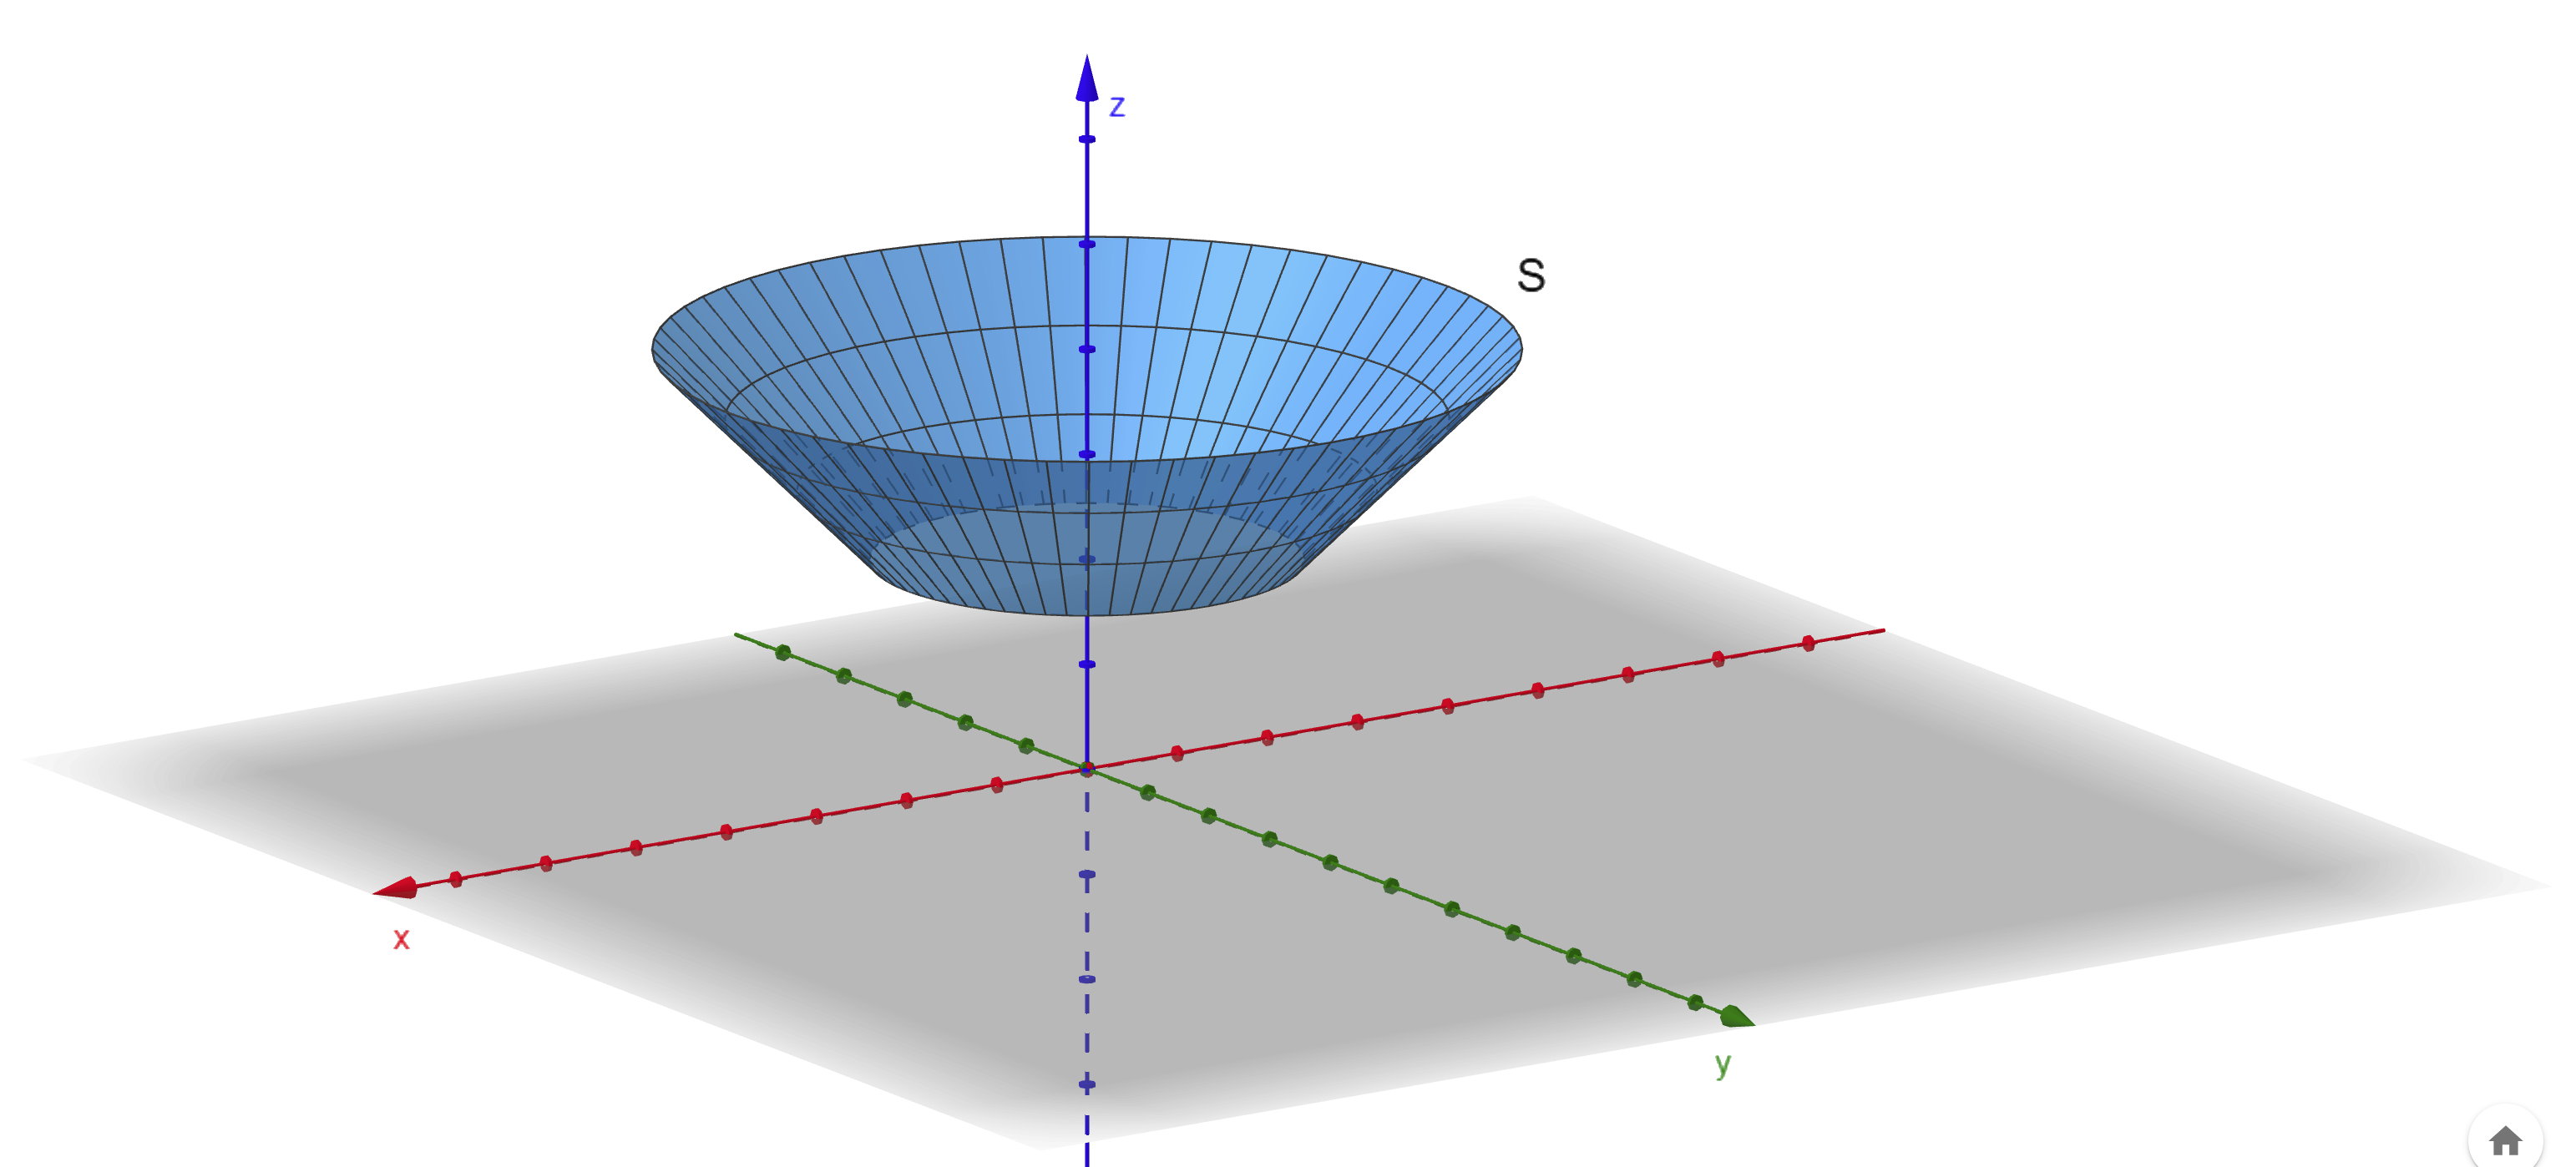
\includegraphics[width=0.5\linewidth]{images/cono1.png}
\end{center}
Calculemos el área de la superficie $S$:\\
$$
    \begin{cases}
        x = r \cos(\theta) \\
        y = r \sin(\theta) \\
        z = r
    \end{cases} \qquad r^2 = x^2 + y^2 = z^2 \implies r = z \qquad \varphi(\theta,z) = \begin{cases}
        x = z \cos(\theta) \\
        y = z \sin(\theta) \\
        z = z
    \end{cases}
$$
$$\overline{D} =[0,2\pi] \times [1,2] \qquad S = \varphi(D)$$
$$ \vec{N}_\varphi = \begin{vmatrix}
        \vec{e}_1      & \vec{e}_2     & \vec{e}_3 \\
        -z\sin(\theta) & z\cos(\theta) & 0         \\
        \cos(\theta)   & \sin(\theta)  & 1
    \end{vmatrix} = (z\cos(\theta), z\sin(\theta), -z)
$$
$$ \lVert \vec{N}_\varphi \rVert^2 = z^2\cos^2(\theta) + z^2\sin^2(\theta) + (-z)^2 = 2z^2 \implies \lVert \vec{N}_\varphi \rVert = z\sqrt{2} \neq 0 \quad \forall (0,z) \in D $$
Entonces $\varphi$ es inyectiva y regular en $D$ (aunque no en $\overline{D}$), luego $S$ es una superficie casi-simple regular.\\
Por último, el área de la superficie $S$ es:
$$ a(S) = \int_{D} \lVert \vec{N}_\varphi \rVert dudv = \int_{\theta = 0}^{\theta = 2\pi} \int_{z = 1}^{z = 2} z\sqrt{2} dz d\theta = \int_{\theta = 0}^{\theta = 2\pi} \left[ \frac{z^2}{2}\sqrt{2} \right]_{1}^{2} d\theta $$
$$= \int_{\theta = 0}^{\theta = 2\pi} \left( \frac{4}{2}\sqrt{2} - \frac{1}{2}\sqrt{2} \right) d\theta = \int_{\theta = 0}^{\theta = 2\pi} \frac{3}{2}\sqrt{2} d\theta = \frac{3}{2}\sqrt{2} \cdot 2\pi = 3\pi\sqrt{2}$$
}

\ejemplo{
    Dada la función $f(x,y,z) = x^2 + y^2 + z^2$, calculemos la integral de superficie de $f$ sobre la superficie $S$ dada por la sección de cono $x^2 + y^2 = z^2, \ 1 < z < 2$ del ejemplo anterior.\\
    Entonces, la integral de superficie de $f$ sobre $S$ es:
    $$ \int_{S} f dS = \int_{D} f(\varphi(\theta,z)) \lVert \vec{N}_\varphi \rVert d\theta dz = \int_{\theta = 0}^{\theta = 2\pi} \int_{z = 1}^{z = 2} 2z^2 \cdot z\sqrt{2} dz d\theta = \int_0^{2\pi} \frac{2\sqrt{2}}{4} \left[ z^4 \right]_1^2 \, d\theta $$
    $$= \int_0^{2\pi} \frac{2\sqrt{2}}{4} (16 - 1) \, d\theta = \int_0^{2\pi} \frac{30\sqrt{2}}{4} \, d\theta = \int_0^{2\pi} \frac{15\sqrt{2}}{2} \, d\theta = \frac{15\sqrt{2}}{2} \cdot (2\pi) = 15\pi\sqrt{2}$$
    Observemos que $\int_{S} f dA = \int_{S} f dS$.
}

\ejemplo{
Área de la esfera en $\mathbb{R}^3$ de radio $R$:
$$ S = \{(x,y,z) \in \mathbb{R}^3 : x^2 + y^2 + z^2 = R^2\} $$
$$ \varphi: U \to \mathbb{R}^3 \qquad \varphi(\theta,\phi) = \begin{cases}
        x = R \cos(\theta)\sin(\phi) \\
        y = R \sin(\theta)\sin(\phi) \\
        z = R \cos(\phi)
    \end{cases} \qquad \overline{D} = \begin{cases}
        \theta \in [0,2\pi] \\
        \phi \in [0,\pi]
    \end{cases}
$$
Entonces, tenemos que $D = (0,2\pi) \times (0,\pi)$ y $\overline{D} = [0,2\pi] \times [0,\pi]$.\\

$$ \vec{N}_\varphi = \begin{vmatrix}
        \vec{e}_1                & \vec{e}_2               & \vec{e}_3    \\
        -R\sin(\theta)\sin(\phi) & R\cos(\theta)\sin(\phi) & 0            \\
        R\cos(\theta)\cos(\phi)  & R\sin(\theta)\cos(\phi) & -R\sin(\phi)
    \end{vmatrix}
$$
$$= R^2 \sin(\phi) \begin{vmatrix}
        \vec{e}_1              & \vec{e}_2              & \vec{e}_3   \\
        -\sin(\theta)          & \cos(\theta)           & 0           \\
        \cos(\theta)\cos(\phi) & \sin(\theta)\cos(\phi) & -\sin(\phi)
    \end{vmatrix} = -R^2 \sin(\phi) \left(\sin{(\phi)} \cos{(\theta)}, \sin{(\phi)} \sin{(\theta)}, \cos{(\phi)}\right) $$
$$ \lVert \vec{N}_\varphi \rVert^2 = R^4 \sin^4(\phi) + R^4 \sin^2(\phi)\cos^2(\phi) = R^4 \sin^2(\phi) \left( \sin^2(\phi) + \cos^2(\phi) \right) = R^4 \sin^2(\phi) $$
$$ \lVert \vec{N}_\varphi \rVert = R^2 \sin(\phi) $$
Luego el área de la esfera es:
$$ a(S) = \int_{D} \lVert \vec{N}_\varphi \rVert dudv = \int_{\theta = 0}^{\theta = 2\pi} \int_{\phi = 0}^{\phi = \pi} R^2 \sin(\phi) d\phi d\theta = \int_{\theta = 0}^{\theta = 2\pi} \left[ -R^2 \cos(\phi) \right]_{0}^{\pi} d\theta $$
$$= \int_{\theta = 0}^{\theta = 2\pi} -R^2 \left((-1) - 1 \right) d\theta = \int_{\theta = 0}^{\theta = 2\pi} 2R^2 d\theta = 2R^2 \cdot (2\pi) = 4\pi R^2$$

}

\subsection{Superficies Regulares a Trozos}

\begin{definición} [Suma de Superficies]
Sean \( S_1, S_2 \subset \mathbb{R}^3 \) dos superficies simples regulares. Se dice que la superficie $S$ es la suma de \( S_1 \) y \( S_2 \), y se denota por \( S = S_1 + S_2 \), si:
\begin{enumerate}
    \item \( S = S_1 \cup S_2 \)
    \item \( S_1 \cap S_2 \subset \partial S_1 \cap \partial S_2 \)
\end{enumerate}
En este caso, se define el borde de \( S \) como:
\[
    \partial S = \overline{(\partial S_1 \cup \partial S_2) \setminus (\partial S_1 \cap \partial S_2)}
\]
Si $\partial S = \emptyset$, entonces se dice que \( S \) no tiene borde y es
cerrada.

Análogamente, se define la suma de superficies $S_1 + S_2 + \ldots + S_k$
siendo cada $S_i$ una superficie simple regular.\\
\end{definición}

\ejemplo{
    Consideramos el cubo $S$ formado por la suma de las superficies de los seis lados del cubo $S = S_1, S_2, \ldots, S_6$. En particular tenemos que $\partial S = \emptyset$.
}

\ejemplo{
    Consideramos ahora el cilindro $S$ formado por la suma de las superficies de los dos "tapas" del cilindro $S_1, S_2$ y la superficie lateral dividida en dos partes iguales $S_3$ y $S_4$. En este caso, tenemos que $S = S_1 + S_2 + S_3 + S_4$, y como en el caso anterior, $\partial S = \emptyset$.
}

\ejemplo{
    Quitémosle una de las tapas al cilindro, entonces tenemos que $S = S_1 + S_2 + S_3$, y en este caso
    $$
        \begin{cases}
            \partial(S_1 + S_2) = C_0 \cup C_1 \\
            \partial S_3 = C_0                 \\
            \partial S = \overline{(\partial(S_1 + S_2) \cup \partial S_3) \setminus (\partial S_1 + S_2) \cap \partial S_3} = \overline{(C_0 \cup C_1 \cup C_0) \setminus (C_0)} = \overline{C_1} = C_1
        \end{cases}
    $$
}
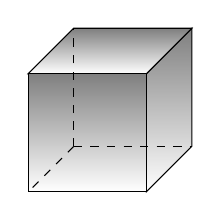
\begin{tikzpicture}[scale=1.5]
    % Caras visibles
    \draw[shade] (1,0,0) -- (1,1,0) -- (1,1,1) -- (1,0,1) -- cycle;
    \draw[shade] (0,1,0) -- (0,1,1) -- (1,1,1) -- (1,1,0) -- cycle;
    \draw[shade] (0,0,1) -- (1,0,1) -- (1,1,1) -- (0,1,1) -- cycle;
    % Lineas traseras
    \draw[dashed] (0,0,0) -- (1,0,0);
    \draw[dashed] (0,0,0) -- (0,1,0);
    \draw[dashed] (0,0,0) -- (0,0,1);
\end{tikzpicture}

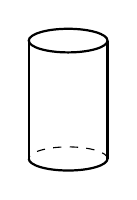
\begin{tikzpicture}[scale=0.5]
    % Cilindro
    \draw[thick] (0,0) ellipse (1 and 0.3);
    \draw[thick] (-1,0) -- (-1,-3);
    \draw[thick] (1,0) -- (1,-3);
    \draw[thick] (-1,-3) arc (180:360:1 and 0.3);
    \draw[dashed] (1,-3) arc (0:180:1 and 0.3);
\end{tikzpicture}

Sea $\vec{F}$ un campo vectorial en $\mathbb{R}^3$ y $S$ una superficie. Nos
preguntamos qué orientación tiene el campo $\vec{F}$ en la superficie $S$.\\
Necesitamos, por tanto, orientar $S$ de alguna forma.

\subsection{Orientación de Superficies}

\begin{definición} [Normal Unitaria de una Superficie]
Sea \( S \) una superficie regular en \( \mathbb{R}^3 \). Una \textbf{normal unitaria} en \( S \) es una función continua
\[
    \vec{n}: S \to \mathbb{R}^3
\]
tal que, para todo punto \( p \in S \), se cumple que \( \vec{n}(p) \) es un
vector \textbf{unitario} y \textbf{normal} a la superficie en \( p \), es
decir:
\[
    \vec{n}(p) \perp T_p(S) \quad \text{y} \quad \|\vec{n}(p)\| = 1,
\]
donde \( T_p(S) \) denota el plano tangente a \( S \) en el punto \( p \).
\end{definición}

\begin{definición} [Superficie Orientada]
Una \textbf{superficie simple regular orientada} es un par \( (S, \vec{n}) \), donde \( S \) es una superficie regular y simple, y \( \vec{n} \) es una normal unitaria que asigna de forma continua a cada punto de \( S \) una orientación consistente.
\end{definición}

\begin{observación}
Una superficie simple y regular admite exactamente dos orientaciones posibles.

Sea \( \varphi : \overline{D} \to S \) una parametrización simple y regular de
\( S \), según la definición adoptada para \( S \). Consideramos el siguiente
campo normal:
\[
    \vec{N}_{\varphi} = \frac{\frac{\partial \varphi}{\partial u} \times \frac{\partial \varphi}{\partial v}}{\left\| \frac{\partial \varphi}{\partial u} \times \frac{\partial \varphi}{\partial v} \right\|}.
\]
\[
    \begin{tikzcd}
        {\overline{D}} \arrow[d, "\vec{n}_\varphi" left]
        \arrow[r, bend left=10, "\varphi"]
        & \operatorname{S}
        \arrow[dl, "\vec{n}"]
        \arrow[l, bend left=10, "\varphi^{-1}"] \\
        {\mathbb{R}^3}
    \end{tikzcd}
\]
Entonces, la función \( \vec{n} = \vec{N}_{\varphi} \circ \varphi^{-1} \)
define una normal unitaria en \( S \), ya que \( \varphi : \overline{D} \to S
\) es un homeomorfismo.

Asimismo, la función \( -\vec{n} : S \to \mathbb{R}^3 \) también es una normal
unitaria en \( S \), lo que muestra que toda superficie simple y regular admite
exactamente dos orientaciones opuestas.

Sean ahora \( \vec{n}_1, \vec{n}_2 : S \to \mathbb{R}^3 \) dos normales
unitarias en \( S \). Definimos la función
\[
    h(p) = \langle \vec{n}_1(p), \vec{n}_2(p) \rangle
\]
para todo \( p \in S \). Esta función \( h : S \to \mathbb{R} \) es continua, y
como \( \vec{n}_1(p) \) y \( \vec{n}_2(p) \) son vectores unitarios, se cumple
que \( |h(p)| = 1 \) para todo \( p \in S \).

Dado que \( S \) es conexa, la imagen de \( h \) debe ser conexa y contenida en
el conjunto \( \{-1, 1\} \). Por tanto, \( h(p) \equiv 1 \) o \( h(p) \equiv -1
\) en toda la superficie. En consecuencia, \( \vec{n}_1 = \vec{n}_2 \) o \(
\vec{n}_1 = -\vec{n}_2 \) en todo \( S \).
\end{observación}

\begin{definición} [Integral de un Campo Vectorial sobre una Superficie]
Sean $(S, \vec{n})$ superficie simple regular orientada y $\vec{F} : S \to \mathbb{R}^3$ un campo vectorial continuo. Se define
$$ \int_{(S, \vec{n})} \vec{F} = \int_{S} \langle \vec{F}, \vec{n} \rangle$$
\end{definición}

\begin{observación}
\vspace{-2.5em}
\begin{enumerate}
    \item $\langle \vec{F}, \vec{n} \rangle$ es un campo escalar continuo en $S$.
    \item Si $\varphi : \overline{D} \to S$ es una parametrización simple regular de $S$
          tal que $\vec{n}_\varphi = \vec{n} \circ \varphi$, $$ \int_{(S, \vec{n})}
              \vec{F} = \int_{S} \langle \vec{F}, \vec{n} \rangle = \int_{D} \langle
              \vec{F}(\varphi(u,v)), \vec{n}_\varphi(u,v) \rangle \lVert \vec{N}_\varphi(u,v)
              \rVert dudv = \int_{D} \langle \vec{F}(\varphi(u,v)), \vec{N}_\varphi(u,v)
              \rangle dudv$$
\end{enumerate}
\end{observación}

\ejemplo{
    Consideremos el paraboloide $S = \{(x,y,z) \in \mathbb{R}^3 : z = x^2 + y^2 \leq 1\}$ y lo orientamos con la normal exterior (la que apunta hacia afuera del vaso).\\
    Sea el campo vectorial $\vec{F}(x,y,z) = (xz,yz,0)$, entonces queremos encontrar la integral de $\vec{F}$ sobre $S$.\\
    $$\overline{D} = \{(x,y) \in \mathbb{R}^2 : x^2 + y^2 \leq 1\} \qquad \partial D = C = \{(x,y) \in \mathbb{R}^2 : x^2 + y^2 = 1\}$$
    Consideramos la parametrización del paraboloide dada por:
    $$ \varphi : \overline{D} \to S \qquad \varphi(x,y) = (x,y,x^2 + y^2)$$
    Nos preguntamos si $\vec{n}_\varphi$ induce la misma orientación que $\vec{n}$.\\
    $$ \vec{N}_\varphi = \begin{vmatrix}
            \vec{e}_1 & \vec{e}_2 & \vec{e}_3 \\
            1         & 0         & 2x        \\
            0         & 1         & 2y        \\
        \end{vmatrix} = (-2x, -2y, 1)$$

    $$ \begin{cases} \vec{N}_\varphi (0,0) = (0,0,1) \\
            \varphi(0,0) = (0,0,0)\end{cases} \quad \text{ que apunta hacia arriba, es decir, hacia dentro del vaso, luego } \vec{n}_\varphi = -\vec{n}
    $$
    $$-\int_{D} \langle \vec{F}(\varphi(x,y)), \vec{N}_\varphi(x,y) \rangle dxdy = -\int_{D} \langle (x(x^2+y^2), y(x^2+y^2), 0), (-2x, -2y, 1) \rangle dxdy $$
    $$= \int_{D} 2x^2(x^2+y^2) + 2y^2(x^2+y^2) dxdy = 2 \int_{D} (x^2+y^2)^2 dxdy $$
    Hacemos el cambio de variables a coordenadas polares:
    $$ x = r \cos(\theta) \qquad y = r \sin(\theta) \qquad dxdy = r dr d\theta $$
    $$ 2\int_{D} (x^2+y^2)^2 dxdy = 2\int_{\theta = 0}^{\theta = 2\pi} \int_{r = 0}^{r = 1} r^4 \cdot r dr d\theta = 2\int_{\theta = 0}^{\theta = 2\pi} \left[ \frac{r^6}{6} \right]_{r = 0}^{r = 1} d\theta = 2\int_{\theta = 0}^{\theta = 2\pi} \frac{1}{6} d\theta = 2\frac{1}{6} (2\pi) = 2\frac{\pi}{3} $$
}

\begin{definición} [Orientación Inducida en el Borde]
Sea \( (S, \vec{n}) \) una superficie simple, regular y orientada, y sea \( \varphi : \overline{D} \to S \) una parametrización regular de \( S \) que preserva la orientación inducida por \( \vec{n} \), es decir, \( \vec{n}_\varphi = \vec{n} \circ \varphi \). Consideramos el borde de \( S \) denotado por \( \partial S = \varphi(\partial D) \).\\
Entonces se define la orientación de \( \partial S \) inducida por \( \vec{n} \) como la que se obtiene al recorrer \( \partial D \) en sentido positivo y proyectar dicho recorrido a \( \partial S \) mediante \( \varphi \), es decir, haciendo la composición \( \varphi \circ \gamma \), donde \( \gamma : [a,b] \to \partial D \) es una parametrización de \( \partial D \) que recorre \( \partial D \) en sentido positivo.
\end{definición}

\begin{observación}
Si \( \gamma : [a,b] \to \partial D \) es una parametrización de \( \partial D \) que recorre esta curva en sentido positivo, entonces la curva \( \varphi \circ \gamma : [a,b] \to \partial S \) recorre \( \partial S \) con la orientación inducida por \( \vec{n} \).

Geométricamente, esto significa que \( \partial S \) se recorre de manera que
el sacacorchos avanza en la dirección de \( \vec{n} \), es decir, si imaginamos
un sacacorchos girando en el sentido del recorrido de \( \partial S \), este se
desplazará en la dirección de \( \vec{n} \).

De manera equivalente, si \( \vec{n} \) representa la vertical en el espacio,
entonces \( \partial S \) se recorre dejando la superficie \( S \) a la
izquierda, lo que coincide con la orientación inducida por \( \vec{n} \).
\end{observación}

\ejemplo{
Dada la superficie $S = \{(x,y,z) \in \mathbb{R}^3 : z = x^2 + y^2 \leq 1\}$ del ejemplo anterior, orientada con la normal exterior, y una parametrización $\varphi : \overline{D} \to S$ dada por $\varphi(x,y) = (x,-y,x^2 + y^2)$, donde $D = \{(x,y) \in \mathbb{R}^2 : x^2 + y^2 \leq 1\}$, veamos que $\vec{n}_\varphi = \vec{n}$.\\
$$ \vec{N}_\varphi = \begin{vmatrix}
        \vec{e}_1 & \vec{e}_2 & \vec{e}_3 \\
        1         & 0         & 2x        \\
        0         & -1        & 2y        \\
    \end{vmatrix} = (-2x, -2y, -1)$$
Haciendo la evaluación $\vec{N}_\varphi (0,0) = (0,0,-1)$, vemos que la normal de $\varphi$ en el punto $(0,0)$ tiene el mismo sentido que $\vec{n}$, es decir, $\vec{n}_\varphi = \vec{n}$, luego $\varphi$ preserva la orientación de $S$.\\
Ahora consideremos una parametrización $\gamma$ de \( C = \partial D = \{(x,y) \in \mathbb{R}^2 : x^2 + y^2 = 1\}\) en sentido positivo (antihorario en el plano \( xy \)), definida por:
\[
    \gamma : [0,2\pi] \to \partial D \qquad \gamma(t) = (\cos t, \sin t), \quad t \in [0, 2\pi].
\]
Fijémonos que la curva definida por $\gamma$ es una curva de Jordan-$C^1$ que
deja el interior de $\partial D$ a la izquierda y el exterior a la derecha, es
decir, es positiva.\\ Componiendo con la transformación \( \varphi \),
obtenemos la curva proyectada en \( S \):
\[
    \varphi \circ \gamma : [0,2\pi] \to \partial S \qquad (\varphi \circ \gamma) (t) = (\cos t, -\sin t, \cos^2 t + \sin^2 t) = (\cos t, -\sin t, 1)
\]
que tiene sentido horario en el plano \( xy \), tal y como se indica en la
figura
\begin{center}
    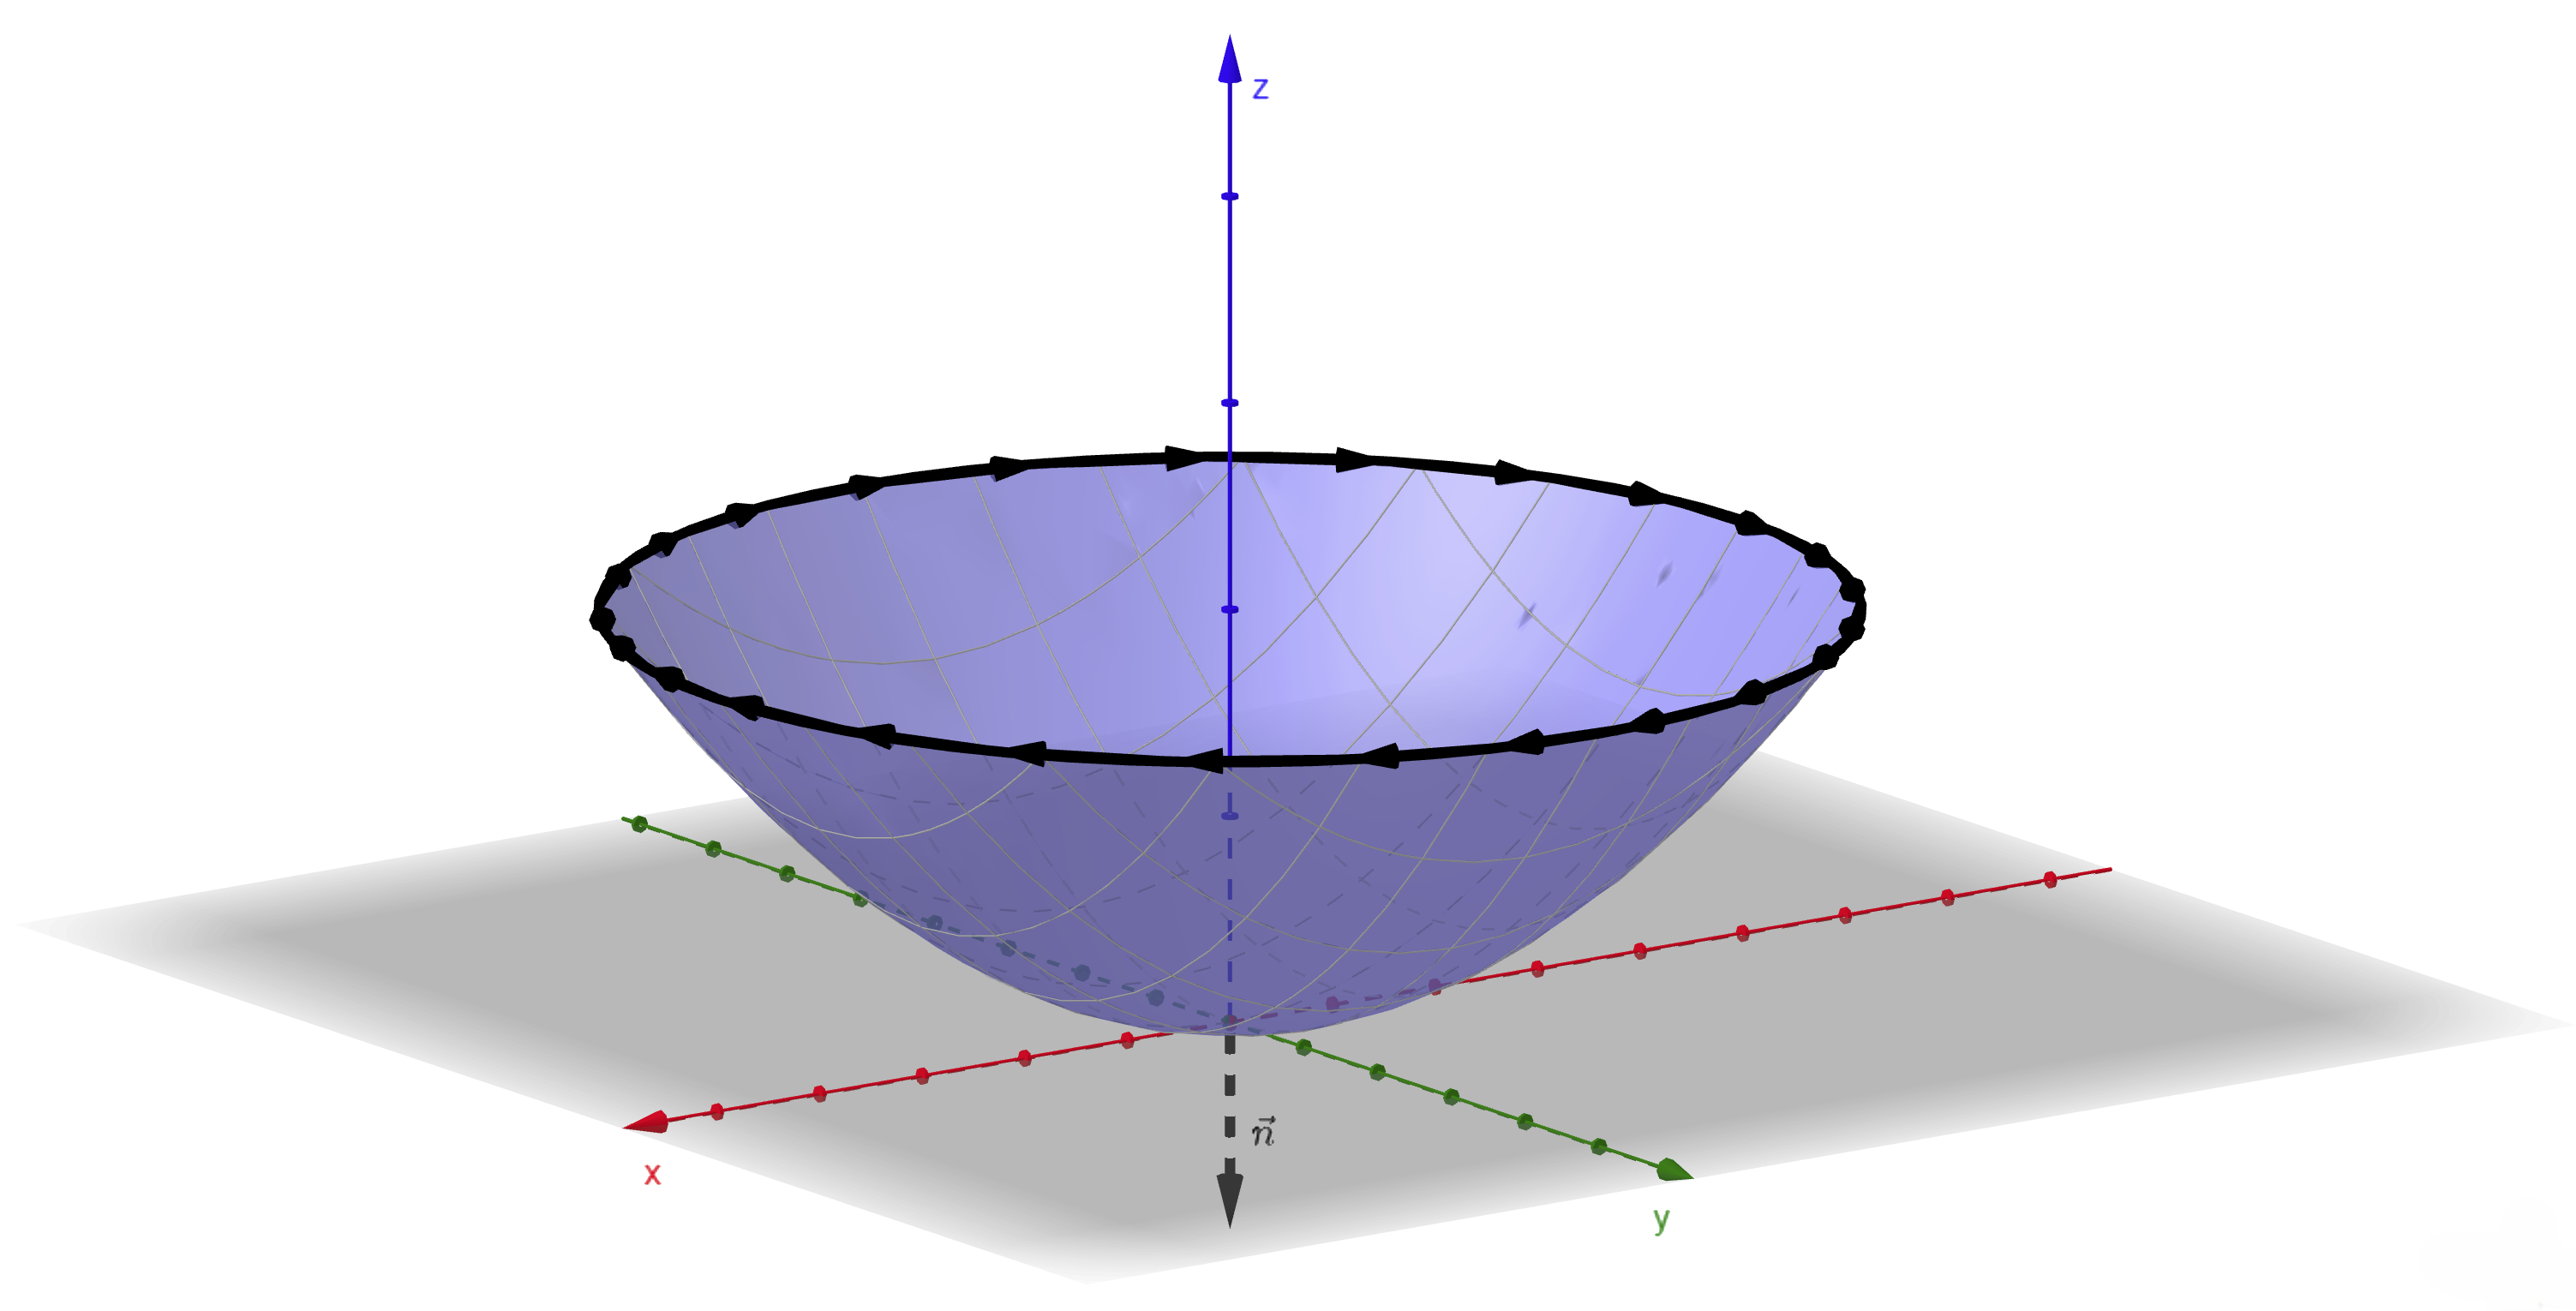
\includegraphics[width=0.6\textwidth]{images/borde1.png}
\end{center}
En efecto, vemos que la orientación inducida por \( \vec{n} \) en \( \partial S \) es la que se obtiene por el recorrido $\varphi \circ \gamma$, al ser composición de una parametrización que preserva la orientación de \( S \) y otra que recorre \( \partial D \) en sentido positivo.\\
Además, observamos que se cumple la regla del sacacorchos, pues si giramos el sacacorchos en el sentido del recorrido de \( \partial S \), este se desplaza hacia abajo, es decir, en la dirección de \( \vec{n} \).\\
Nótese que tomando el vector normal $\vec{n} = (0,0,-1)$ como referencia de eje vertical, al recorrer $\partial S$ con $\varphi \circ \gamma$, la superficie \( S \) queda a la izquierda.
}

\begin{definición} [Orientación Compatible]
Sean \( (S_1, \vec{n}_1) \) y \( (S_2, \vec{n}_2) \) dos superficies simples y regulares de manera que \( S = S_1 + S_2 \), entonces se dice que $\vec{n}_1$ y $\vec{n}_2$ son compatibles si inducen orientaciones opuestas en $\partial S_1 \cap \partial S_2$.\\
En este caso, se dice que $\vec{n} = (\vec{n}_1, \vec{n}_2)$ establece una orientación en $\partial S$ que se llama orientación inducida por $(\vec{n}_1, \vec{n}_2)$.\\
Se dice que $S = S_1 + S_2$ es orientable si $S_1$ y $S_2$ admiten orientaciones compatibles.\
Análogamente, de manera recursiva, si $S = S_1 + S_2 + \ldots + S_k$ donde $(S_i, \vec{n}_i)$ son superficies orientadas, se define $(\vec{n}_1, \ldots, \vec{n}_k)$ como compatible si las orientaciones inducidas por $(\vec{n}_1, \ldots, \vec{n}_{k-1})$ en $S_1 + S_2 + \ldots + S_{k-1}$ y $\vec{n}_k$ en $S_k$ son opuestas en $\partial (S_1 + S_2 + \ldots + S_{k-1}) \cap \partial S_k$.
\end{definición}

\ejemplo{
    Consideremos el cilindro $(S,\vec{n}) = (S_1,\vec{n}_1) + (S_2,\vec{n}_2)$ sin tapas con la orientación exterior.
    $$ S = \{(x,y,z) \in \mathbb{R}^3 : x^2 + y^2 = 1, \ z \in [0,1] \} $$
    donde
    $$ S_1 = \{(x,y,z) \in \mathbb{R}^3 : x^2 + y^2 = 1, \ 0 \leq y, \ z \in [0,1] \}$$
    $$S_2 = \{(x,y,z) \in \mathbb{R}^3 : x^2 + y^2 = 1, \ y \leq 0, \ z \in [0,1] \} $$
    La representación gráfica de $S$ es la siguiente:
    \begin{center}
        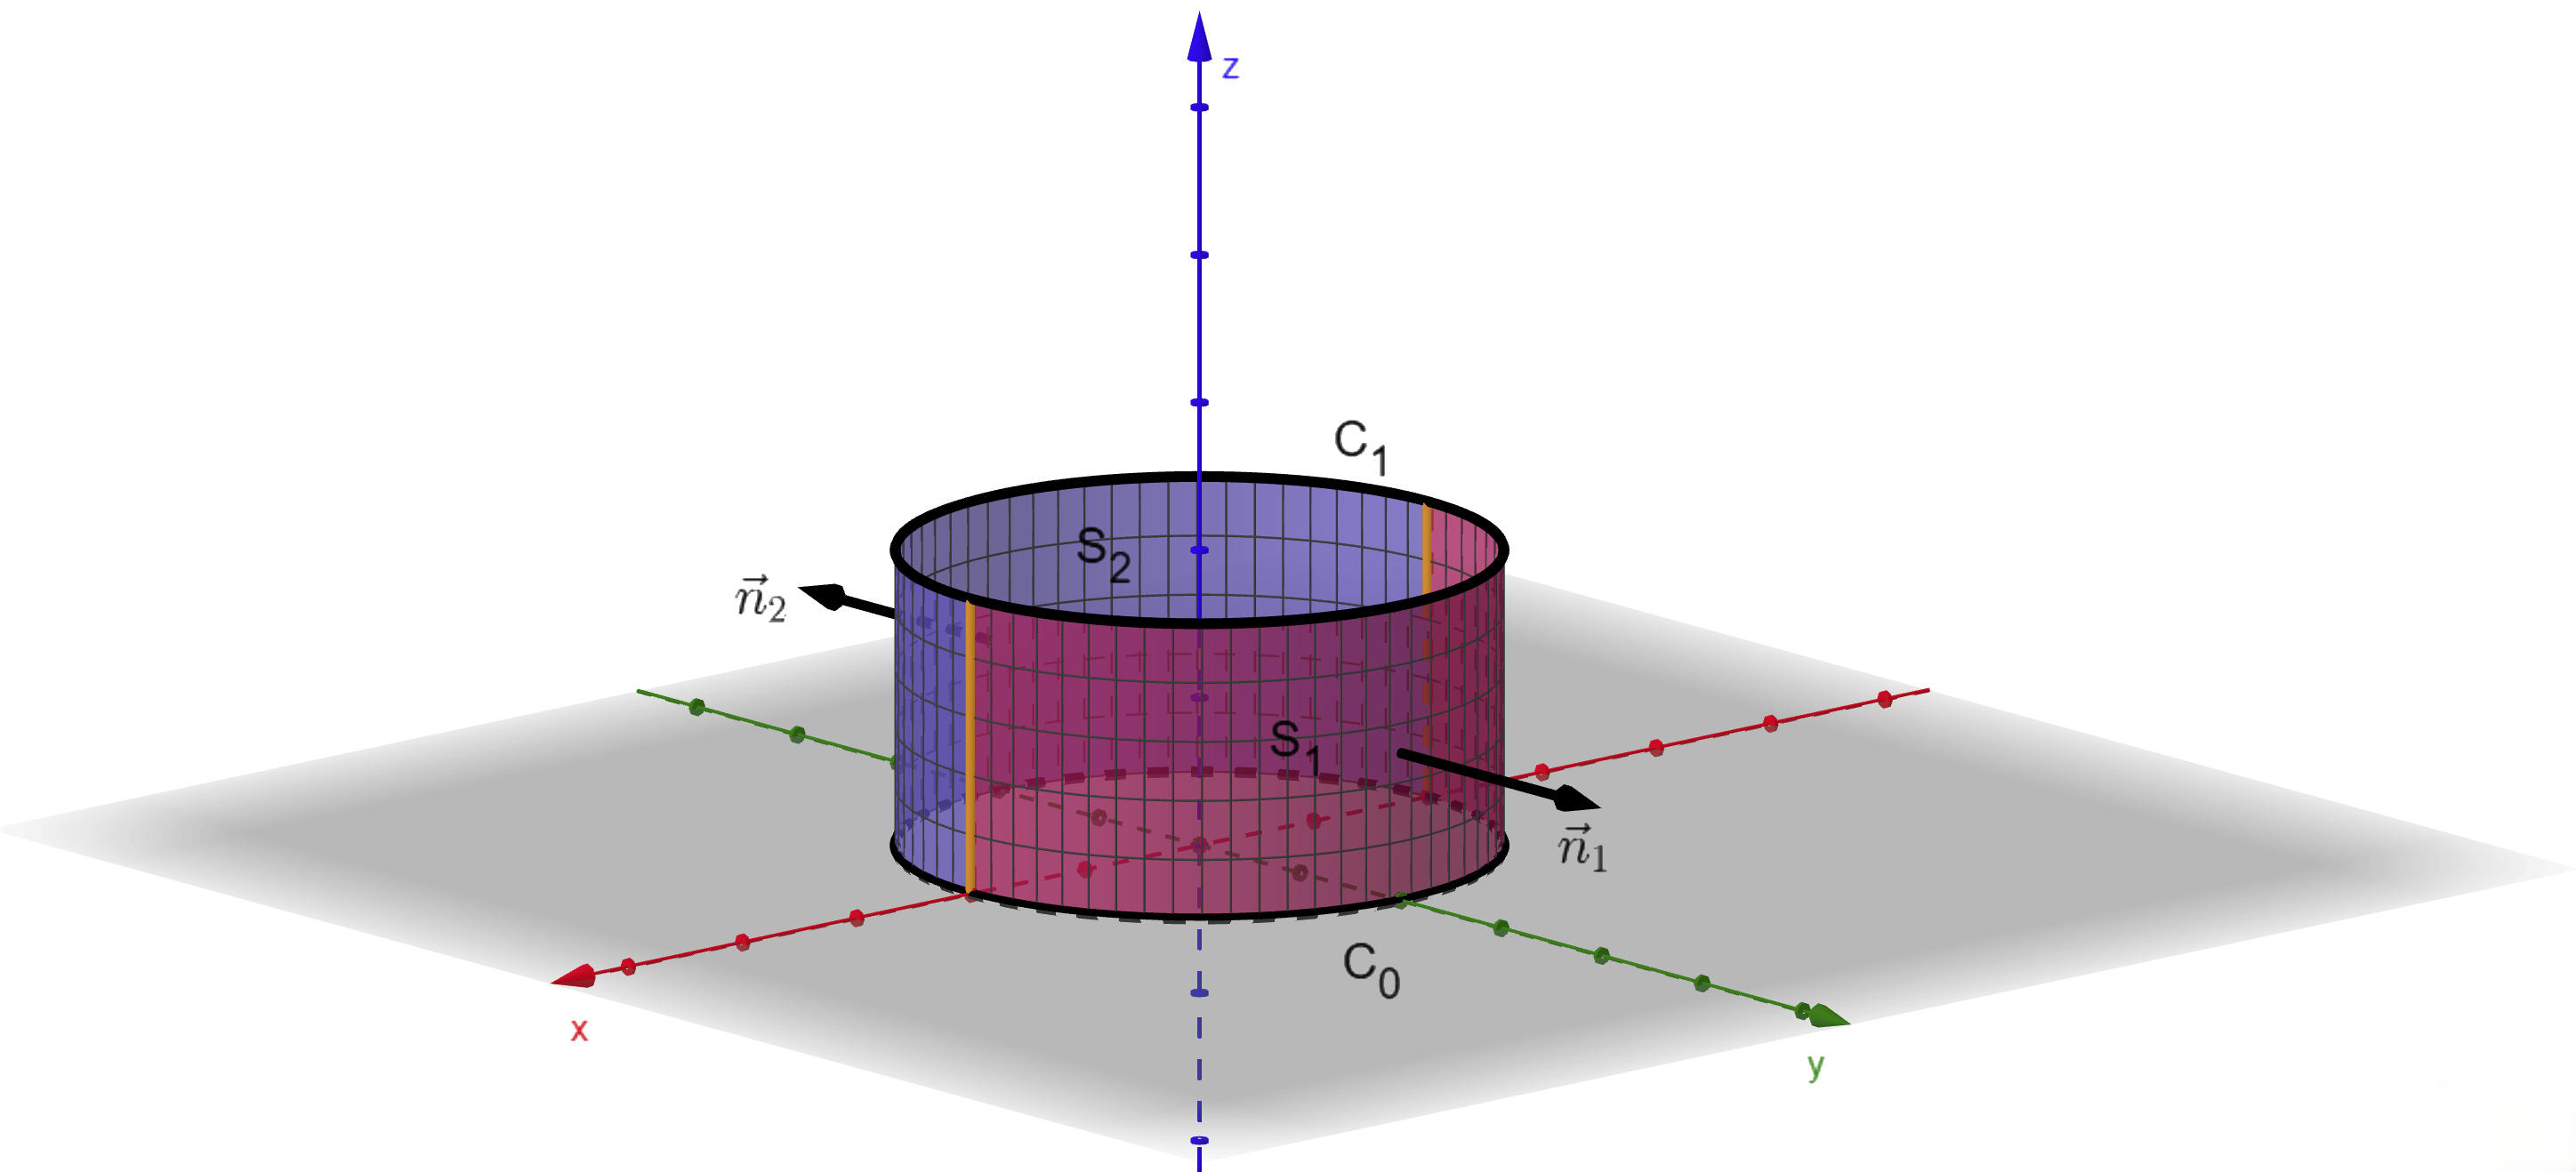
\includegraphics[width=0.65\linewidth]{images/cilindrocompuesto.png}
    \end{center}
    donde $C_0 = \{(x,y,z) \in \mathbb{R}^3 : x^2 + y^2 = 1, \ z = 0\}$ y $C_1 = \{(x,y,z) \in \mathbb{R}^3 : x^2 + y^2 = 1, \ z = 1\}$ son las tapas del cilindro. En particular tenemos que $\partial S = C_0 \cup C_1$.\\
    Veamos que $\vec{n}_1$ y $\vec{n}_2$ son compatibles y que, por tanto, $S$ es orientable siendo $\vec{n} = (\vec{n}_1, \vec{n}_2)$ la orientación inducida en $S$.\\
    Para ello, veamos las orientaciones que inducen $\vec{n}_1$ y $\vec{n}_2$ en $\partial S_1$ y $\partial S_2$ respectivamente. En efecto, por la regla del sacacorchos, las orientaciones inducidas serán las descritas por las siguientes figuras:
    \begin{center}
        \begin{minipage}{0.48\textwidth}
            \centering
            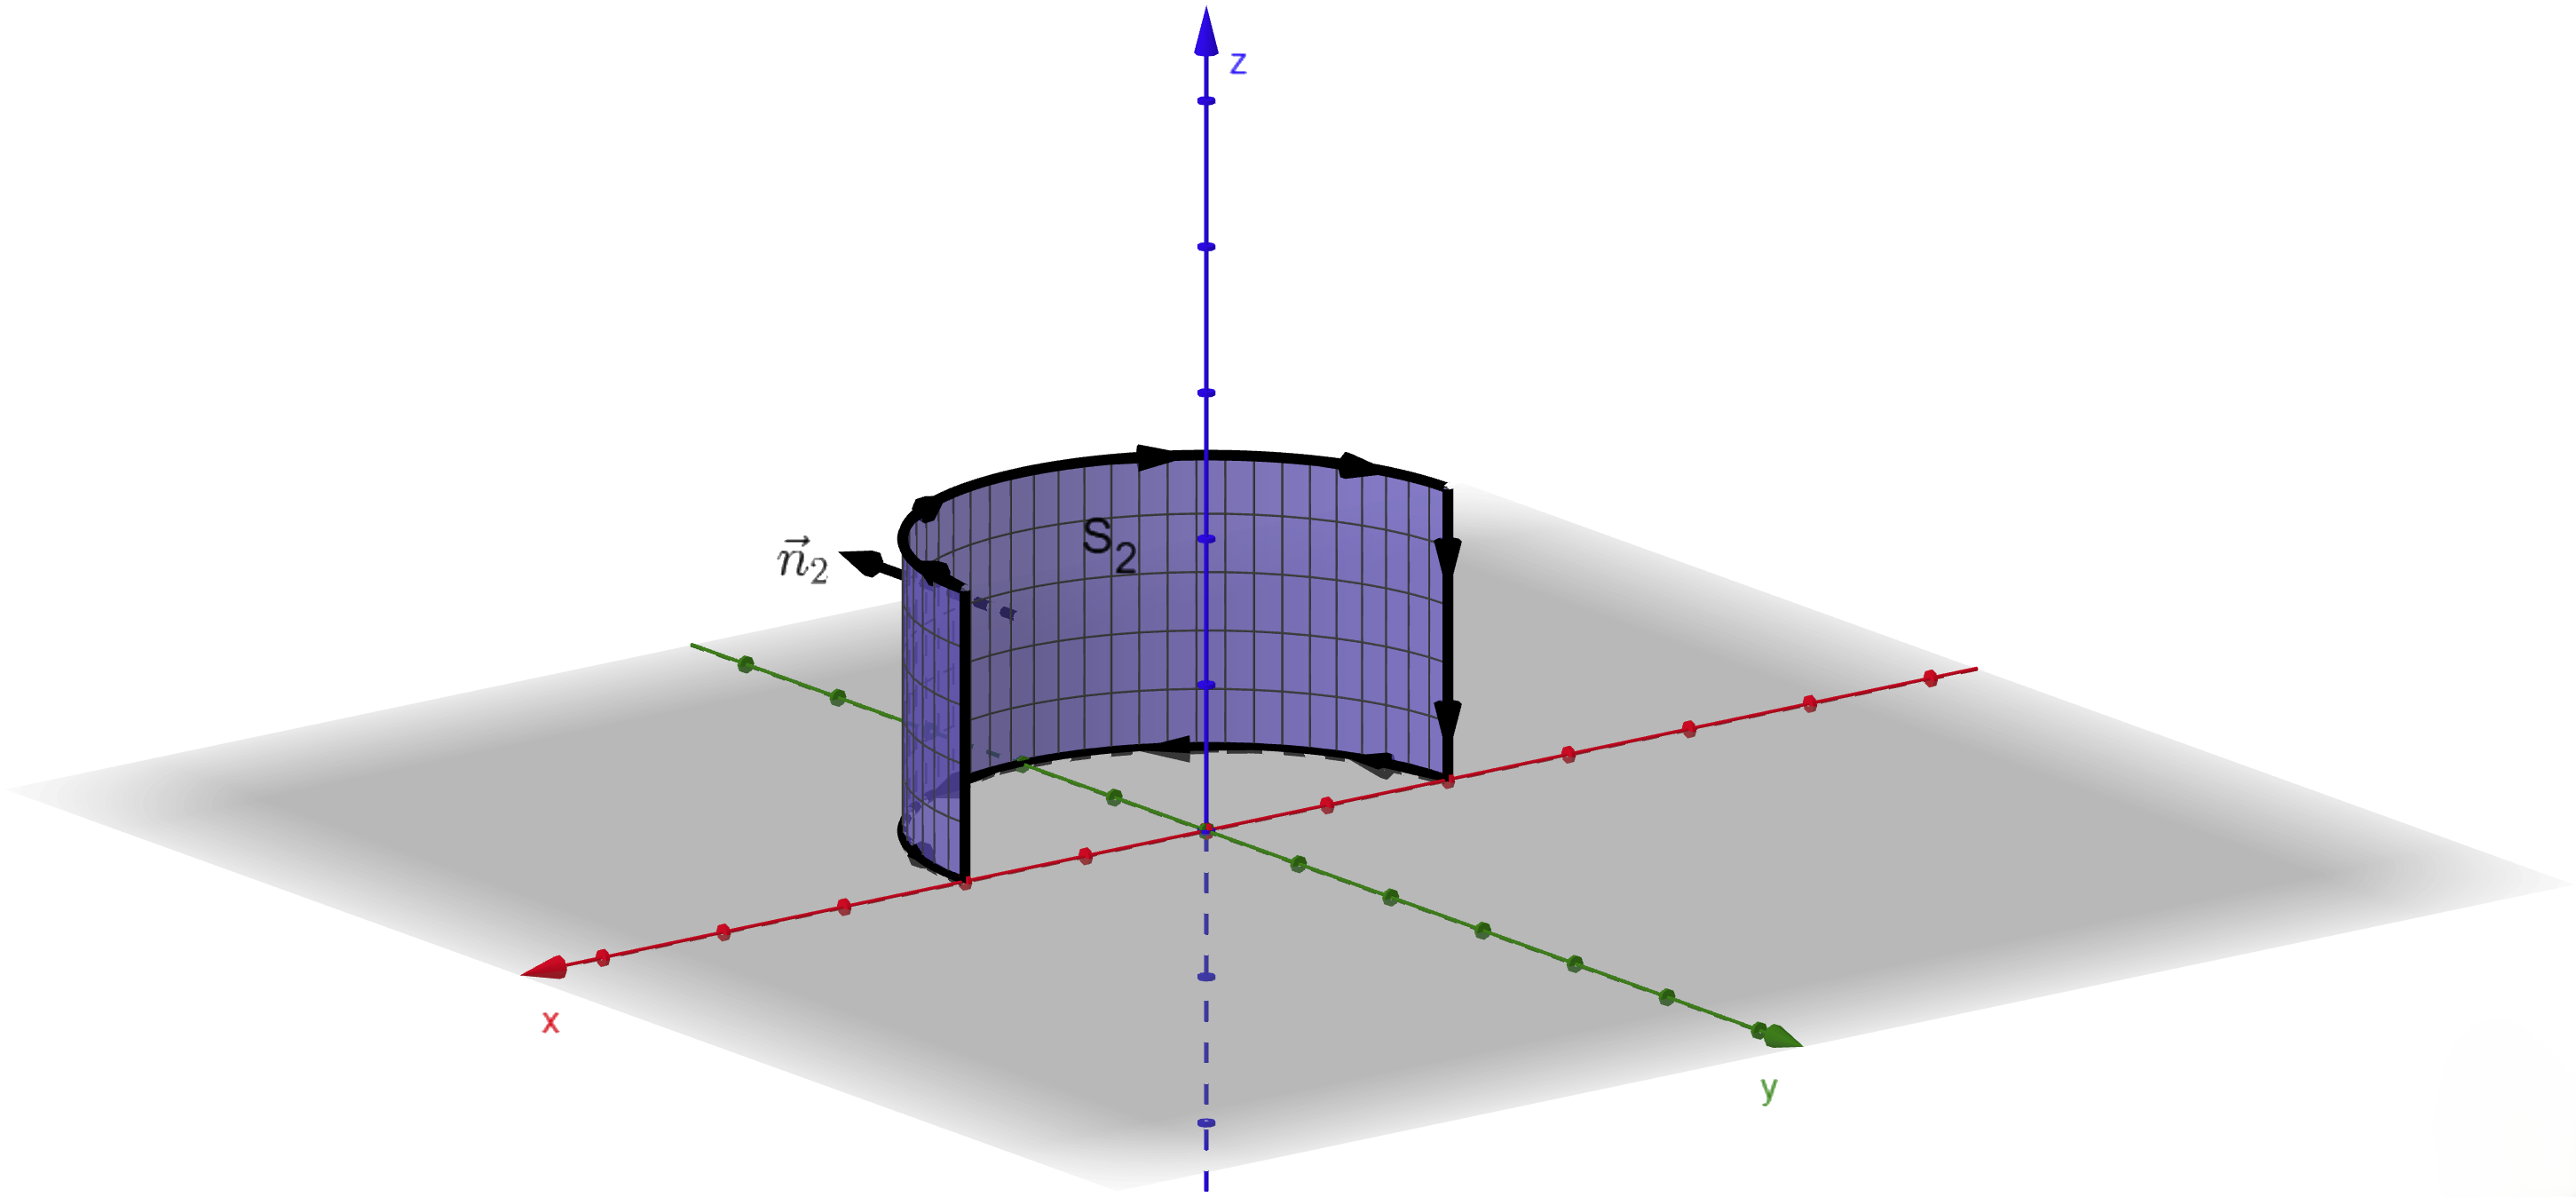
\includegraphics[width=\linewidth]{images/half1.png}
        \end{minipage}
        \hfill
        \begin{minipage}{0.48\textwidth}
            \centering
            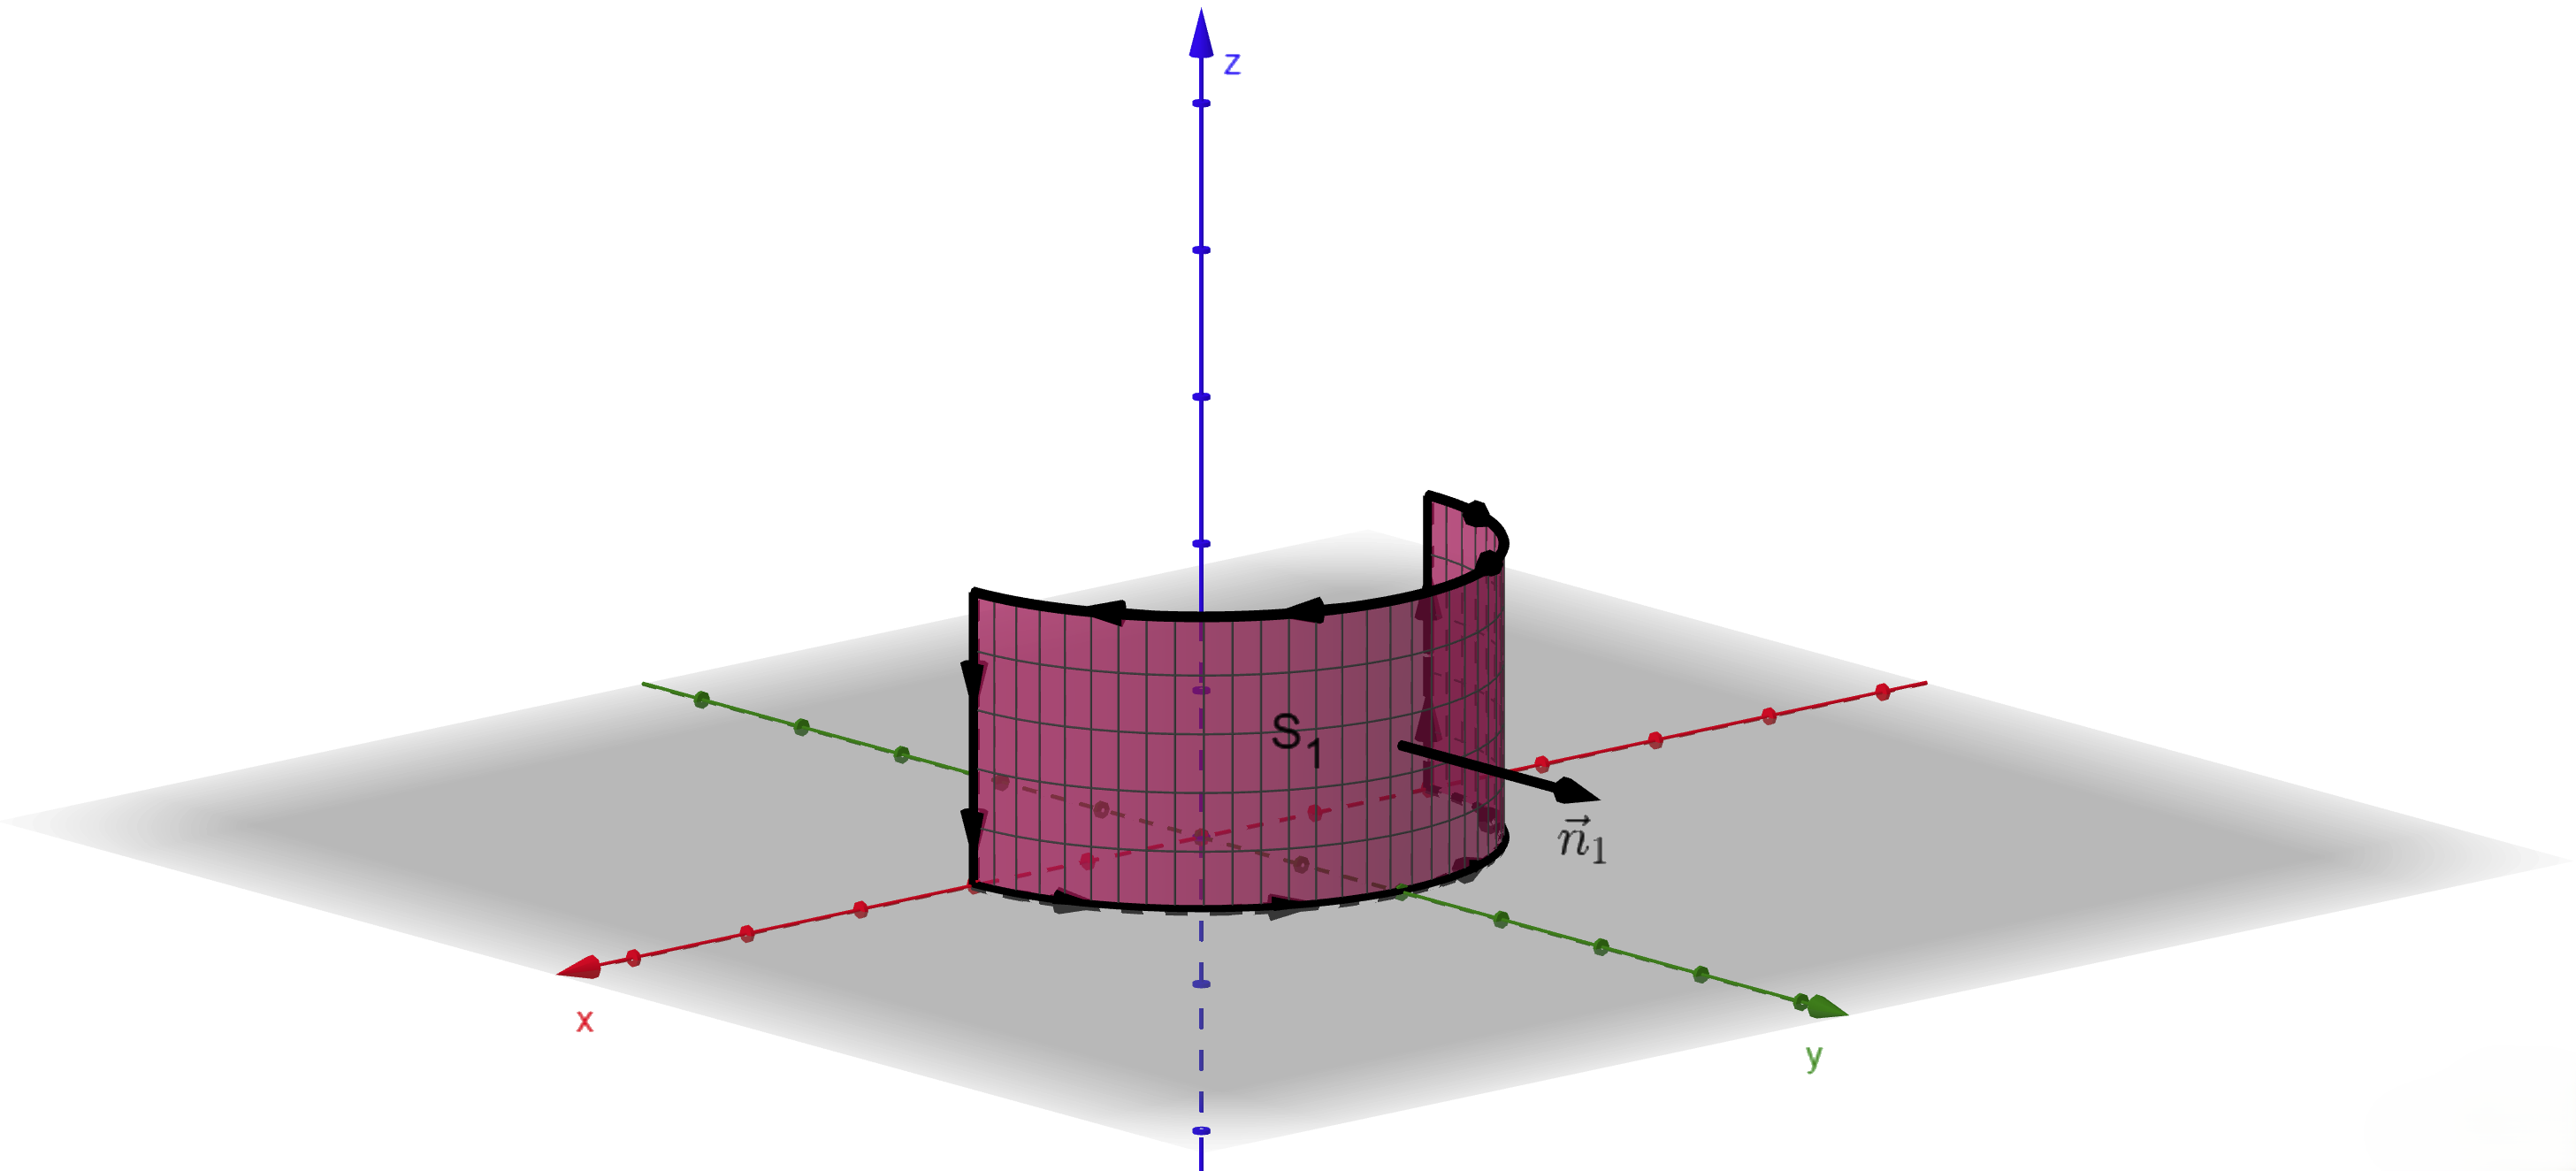
\includegraphics[width=\linewidth]{images/half2.png}
        \end{minipage}
    \end{center}
    Además en la intersección de los bordes $\partial S_1 \cap \partial S_2$ (parte naranja de la primera figura), las orientaciones inducidas son opuestas, luego $\vec{n}_1$ y $\vec{n}_2$ son compatibles, es decir, $S$ es orientable.\\
    Teniendo en cuenta la orientación inducida en el borde de $S_1$ y $S_2$, consideramos dos parametrizaciones $\gamma_0$ y $\gamma_1$ de $C_0$ y $C_1$ respectivamente:
    $$
        \begin{cases}
            \gamma_0(t) = (\cos(t), \sin(t), 0) \quad 0 \leq t \leq 2\pi  \\
            \gamma_1(t) = (-\cos(t), \sin(t), 1) \quad 0 \leq t \leq 2\pi \\
        \end{cases}
    $$
    donde $\gamma_1$ recorre negativamente $C_1$ y $\gamma_0$ positivamente $C_0$, luego $\partial S = C_0^+ \cup C_1^-$.

}

\ejemplo{
    Consideramos ahora el cilindro del ejemplo anterior pero con la tapa de abajo:
    $$ S = \{(x,y,z) \in \mathbb{R}^3 : x^2 + y^2 = 1, \ z \in [0,1] \} $$
    $$ S = \underbrace{S_1 + S_3}_{S_0} + S_3 \text{ donde } S_3 = \{(x,y,z) \in \mathbb{R}^3 : x^2 + y^2 \leq 1, \ z = 0 \} $$
    \begin{center}
        \begin{minipage}{0.48\textwidth}
            \centering
            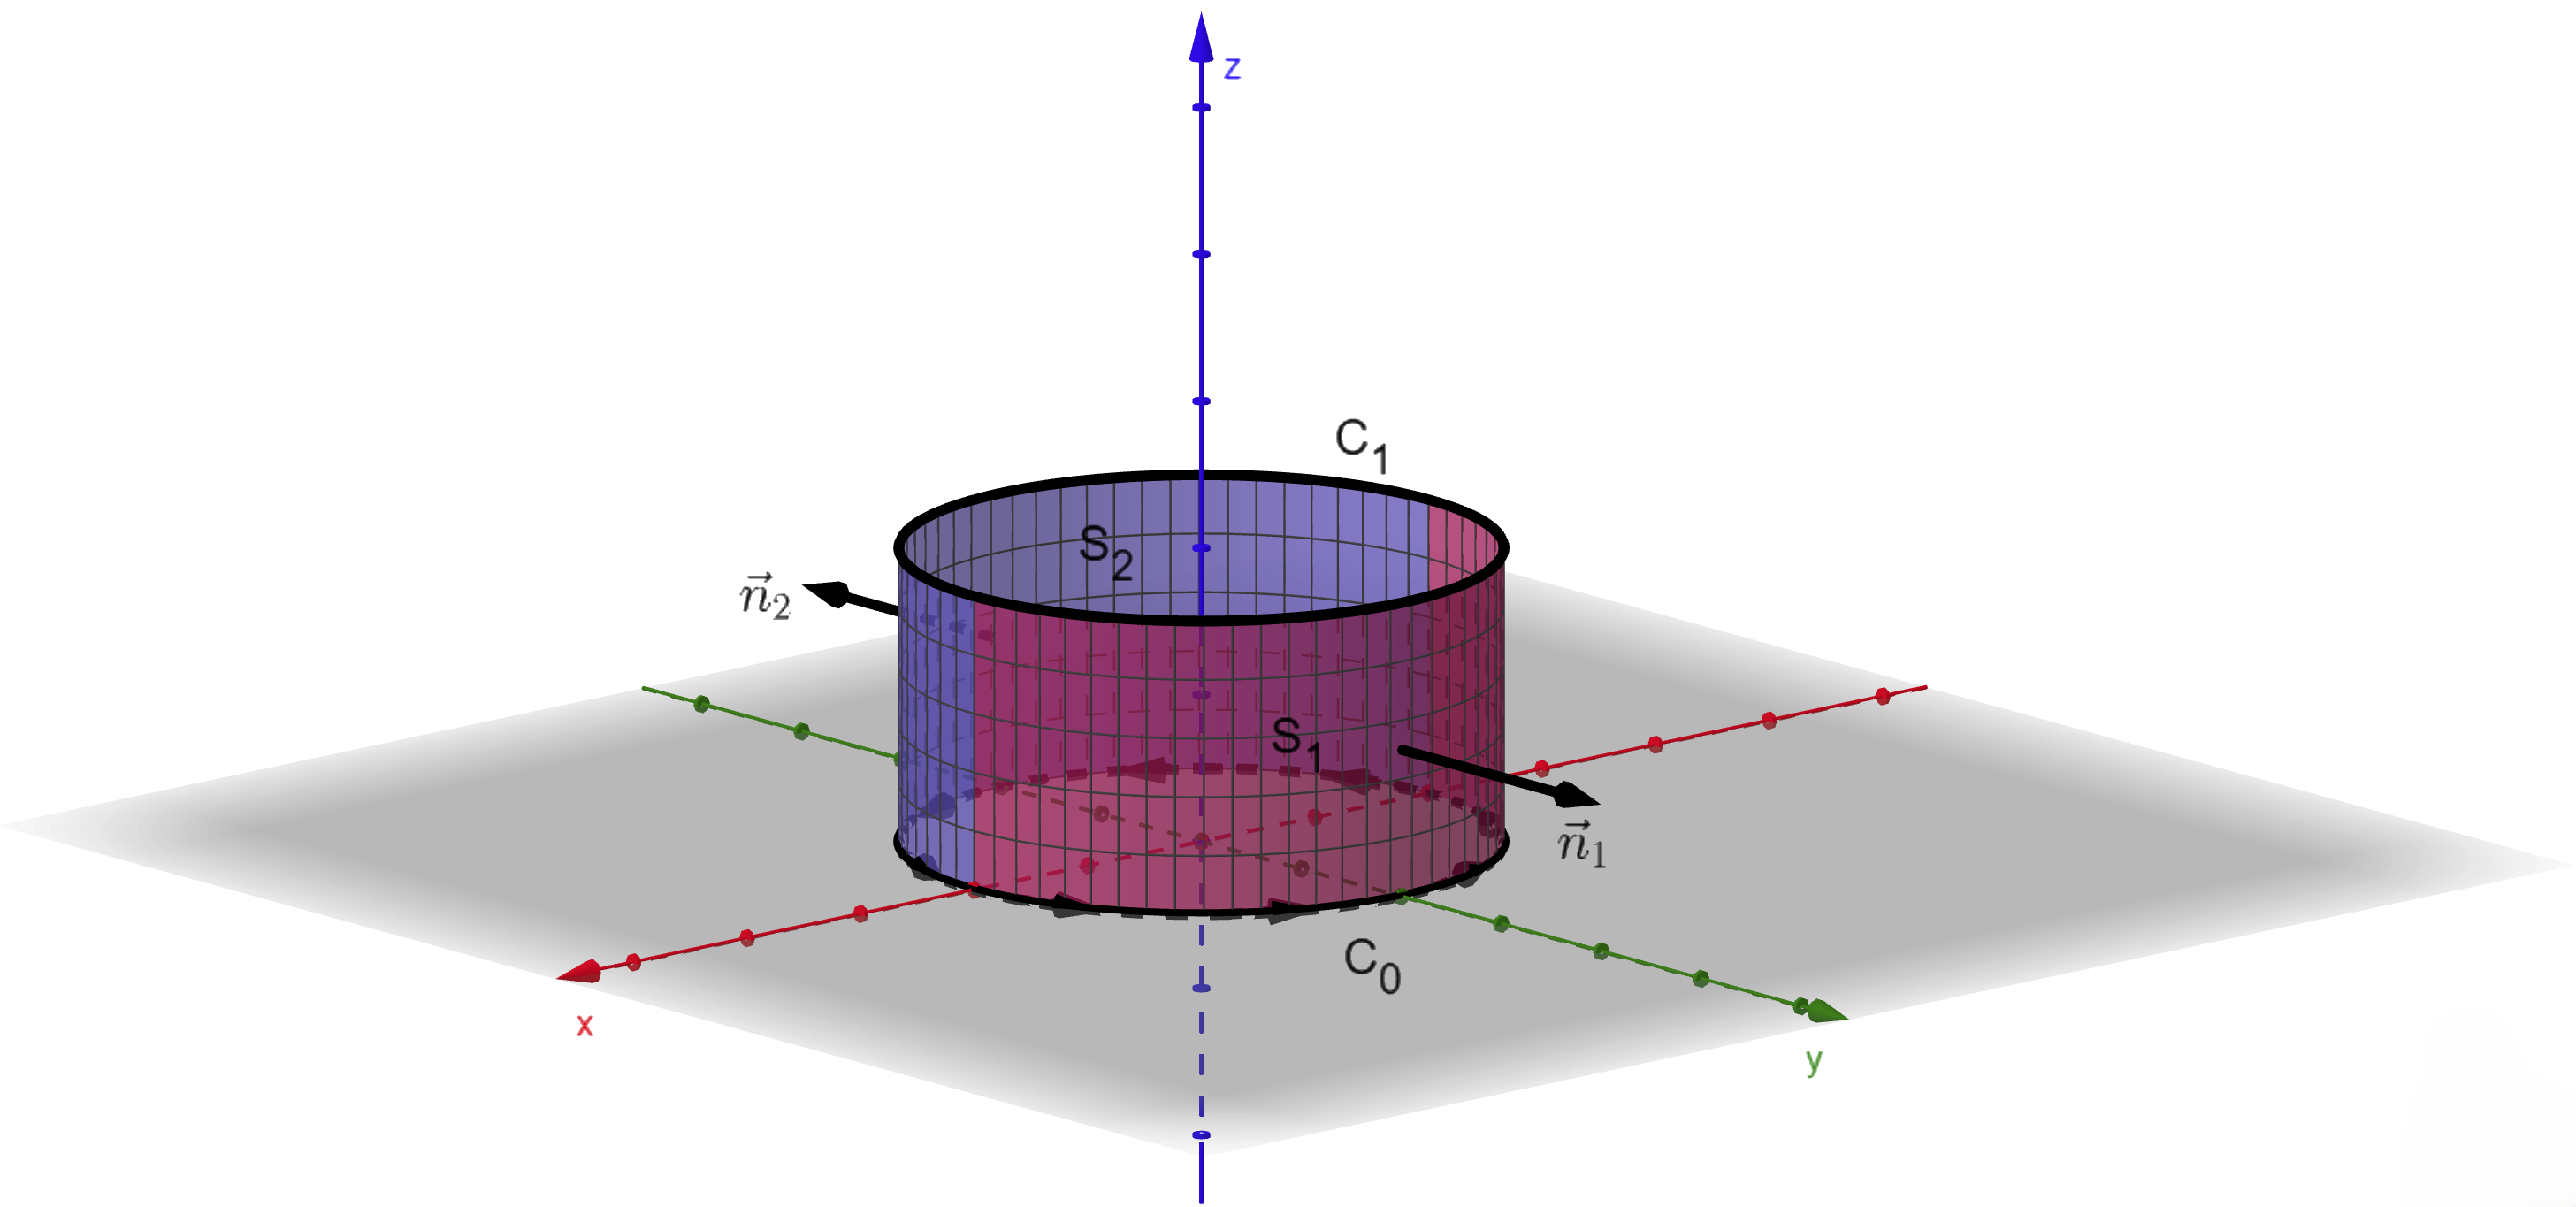
\includegraphics[width=\linewidth]{images/cilindro3.png}
        \end{minipage}
        \hfill
        \begin{minipage}{0.48\textwidth}
            \centering
            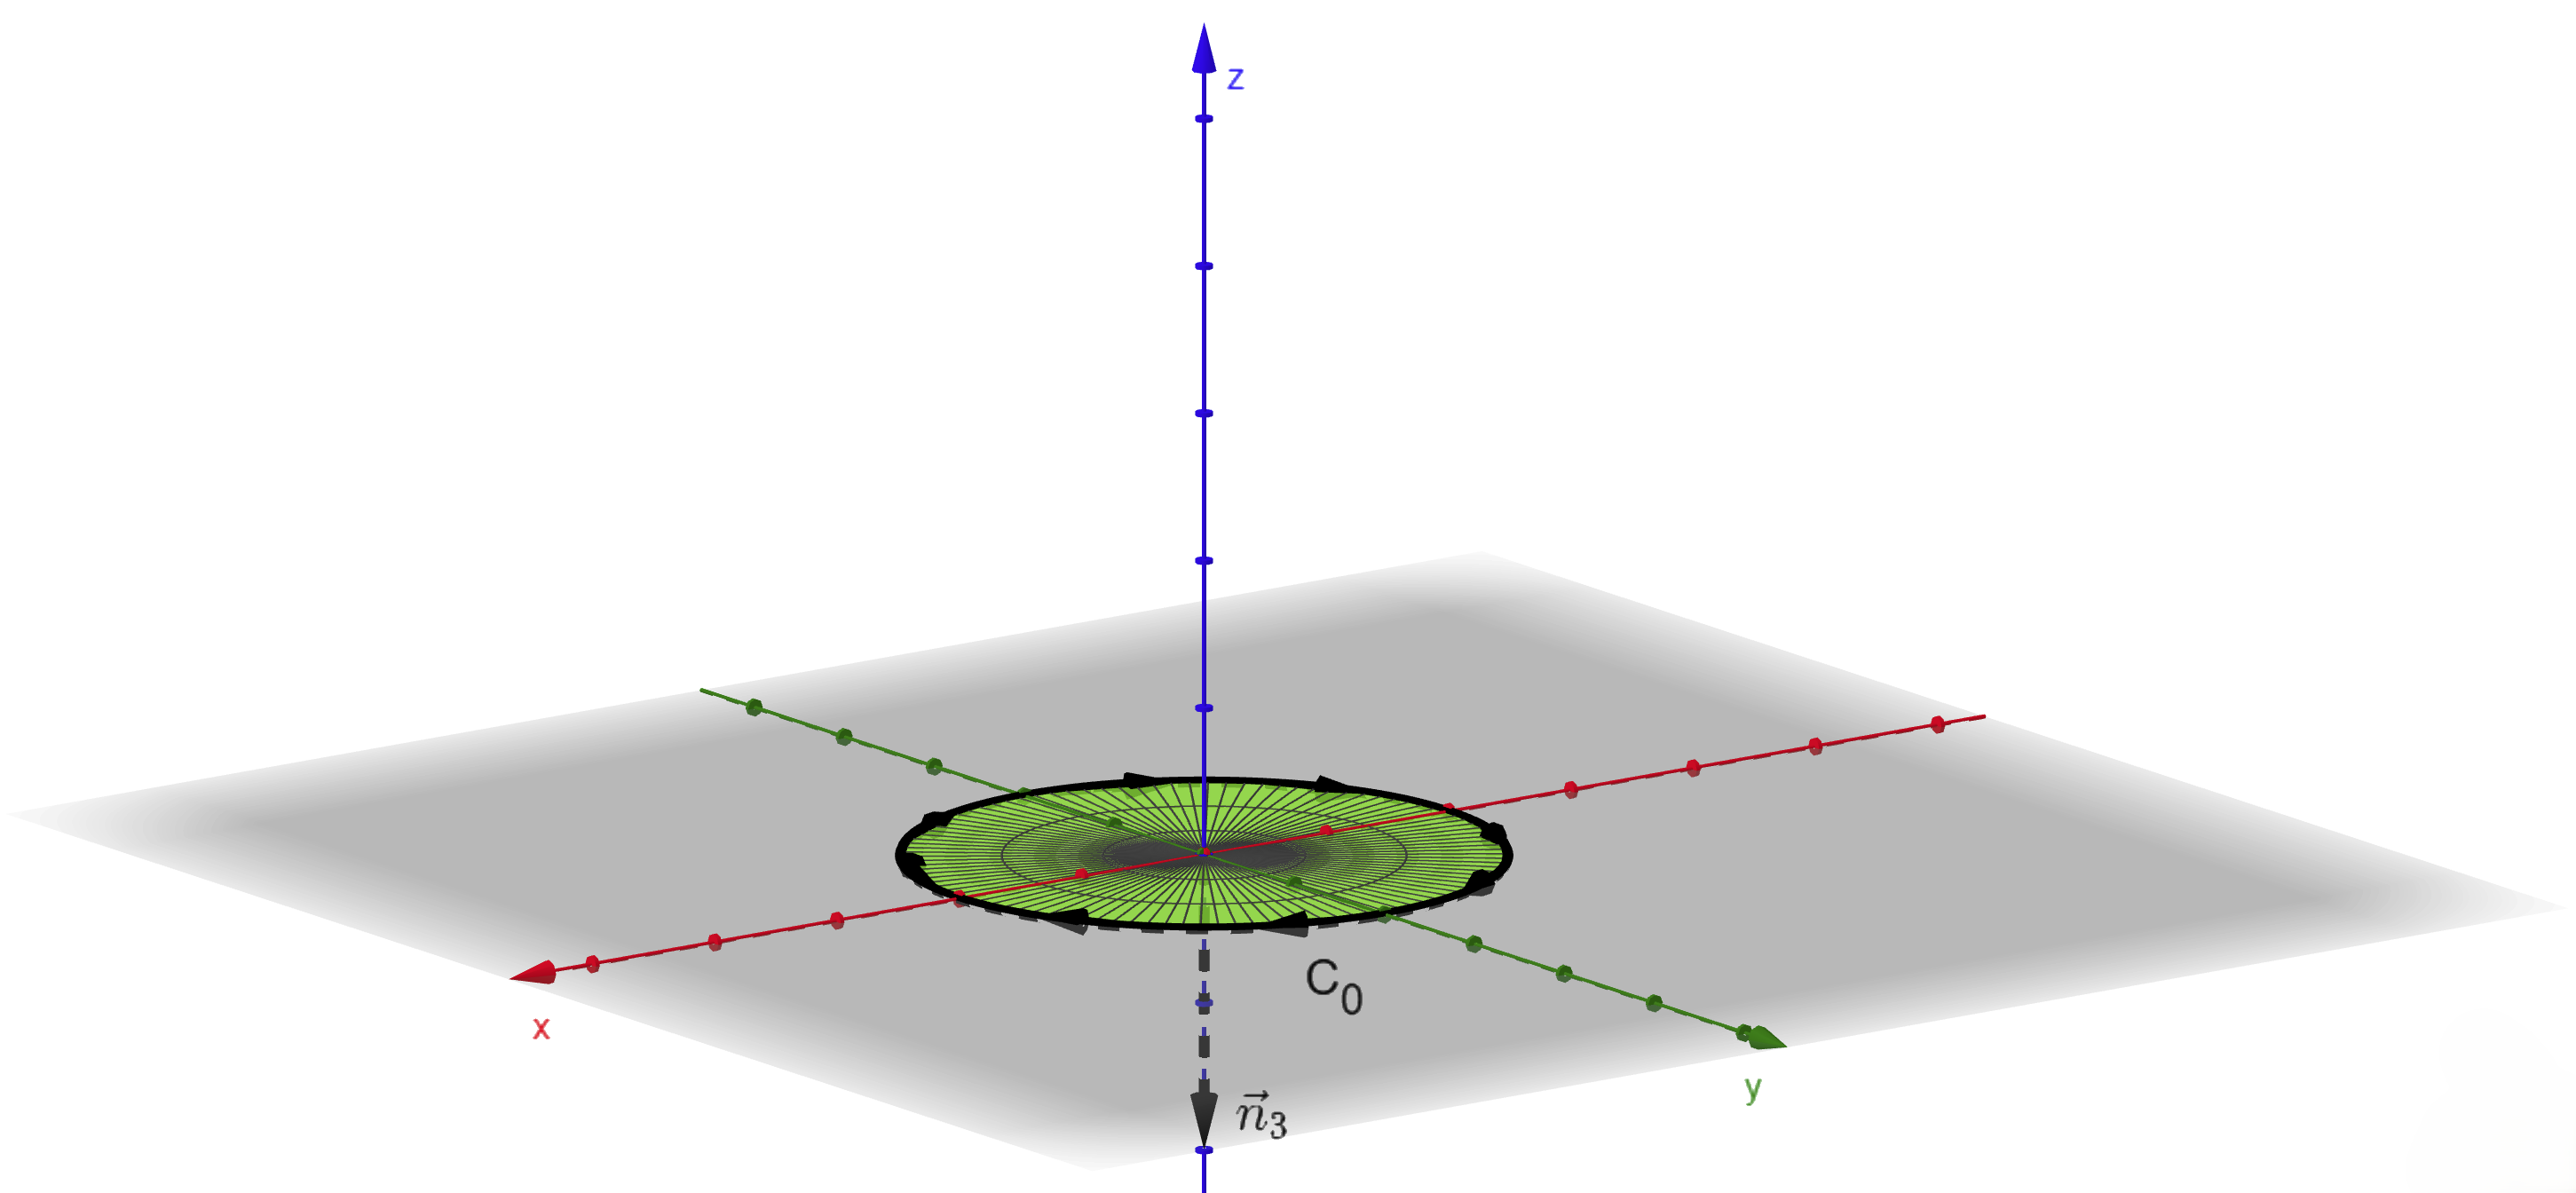
\includegraphics[width=\linewidth]{images/tapa1.png}
        \end{minipage}
    \end{center}
    Consideramos $\vec{n}_3$ normal hacia abajo en $S_3$ y obtenemos que $\vec{n}_3$ induce en $\partial S_3 = C_0$ la orientación opuesta a la de $S_0$, luego son compatibles. Lo mismo podemos hacer con la tapa de arriba, y así obtenemos el cilindro completo, que es orientable con $\partial S = \emptyset$.
}

\textbf{Superficies no orientables:}
\begin{multicols}{3}  % Start a 3-column environment
    \begin{enumerate}
        \item Banda de Moebius
              \begin{center}
                  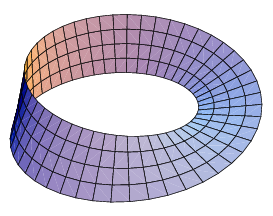
\includegraphics[width=0.7\linewidth]{images/moebius.png}
              \end{center}

        \item Plano proyectivo
              \begin{center}
                  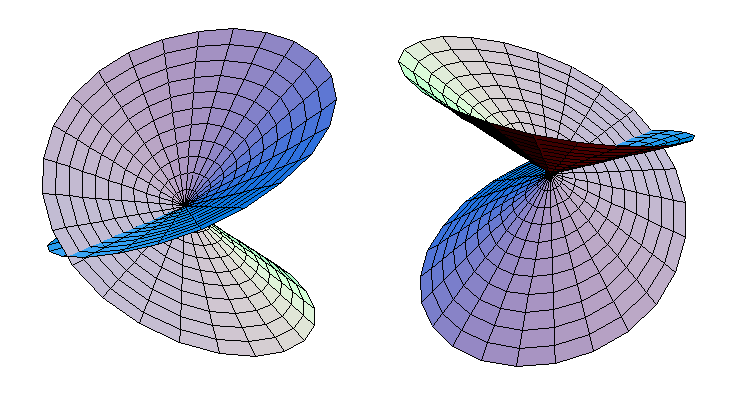
\includegraphics[width=1\linewidth]{images/SelfIntersectingDisk.png}
              \end{center}
        \item Botella de Klein
              \begin{center}
                  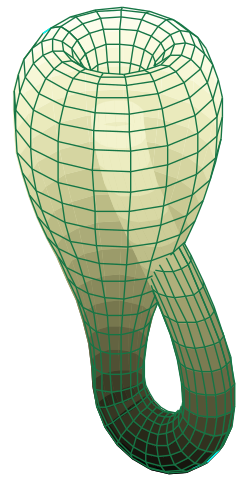
\includegraphics[width=0.3\linewidth]{images/Klein.png}
              \end{center}
    \end{enumerate}
\end{multicols}

\begin{definición} [Integral de Superficie Orientada Regular a Trozos]
Sea $(S, \vec{n})$ una superficie simple, regular a trozos y orientada, es decir, $S = S_1 + S_2 + \ldots + S_k$ donde $(S_i, \vec{n}_i)$ son superficies simples , regulares y orientadas para $i = 1, \ldots, k$, con $(\vec{n}_1, \ldots, \vec{n}_k)$ orientaciones compatibles.\\
Sea $\vec{F} : S \to \mathbb{R}^3$ un campo vectorial continuo. Se define entonces
$$ \int_{(S, \vec{n})} \vec{F} = \sum_{i=1}^{k} \int_{(S_i, \vec{n}_i)} \vec{F} $$
\end{definición}

\ejemplo{
    Sea \( S = S_1 \cup S_2 \), donde:
    \[
        S_1 = \left\{ (x, y, z) \in \mathbb{R}^3 \mid x^2 + y^2 = z,\ z \in [0,1] \right\}, \quad
        S_2 = \left\{ (x, y, z) \in \mathbb{R}^3 \mid x^2 + y^2 \leq 1,\ z = 1 \right\}
    \]
    y sea \( \vec{n} \) el campo normal exterior. Consideramos el campo vectorial
    \( \vec{F}(x, y, z) = (xz,\ yz,\ 0) \), y queremos calcular la integral de \(
    \vec{F} \) sobre la superficie \( S \):
    \[
        \int_S \vec{F} \cdot \vec{n}
    \]
    Aplicando la regla del sacacorchos (regla de la mano derecha), observamos que
    las superficies orientadas \( (S_1, \vec{n}_1) \) y \( (S_2, \vec{n}_2) \)
    inducen sobre la curva
    \[
        C = \partial S_1 \cap \partial S_2 = \left\{ (x, y, z) \in \mathbb{R}^3 \mid x^2 + y^2 = 1,\ z = 1 \right\}
    \]
    orientaciones opuestas.

    \begin{center}
        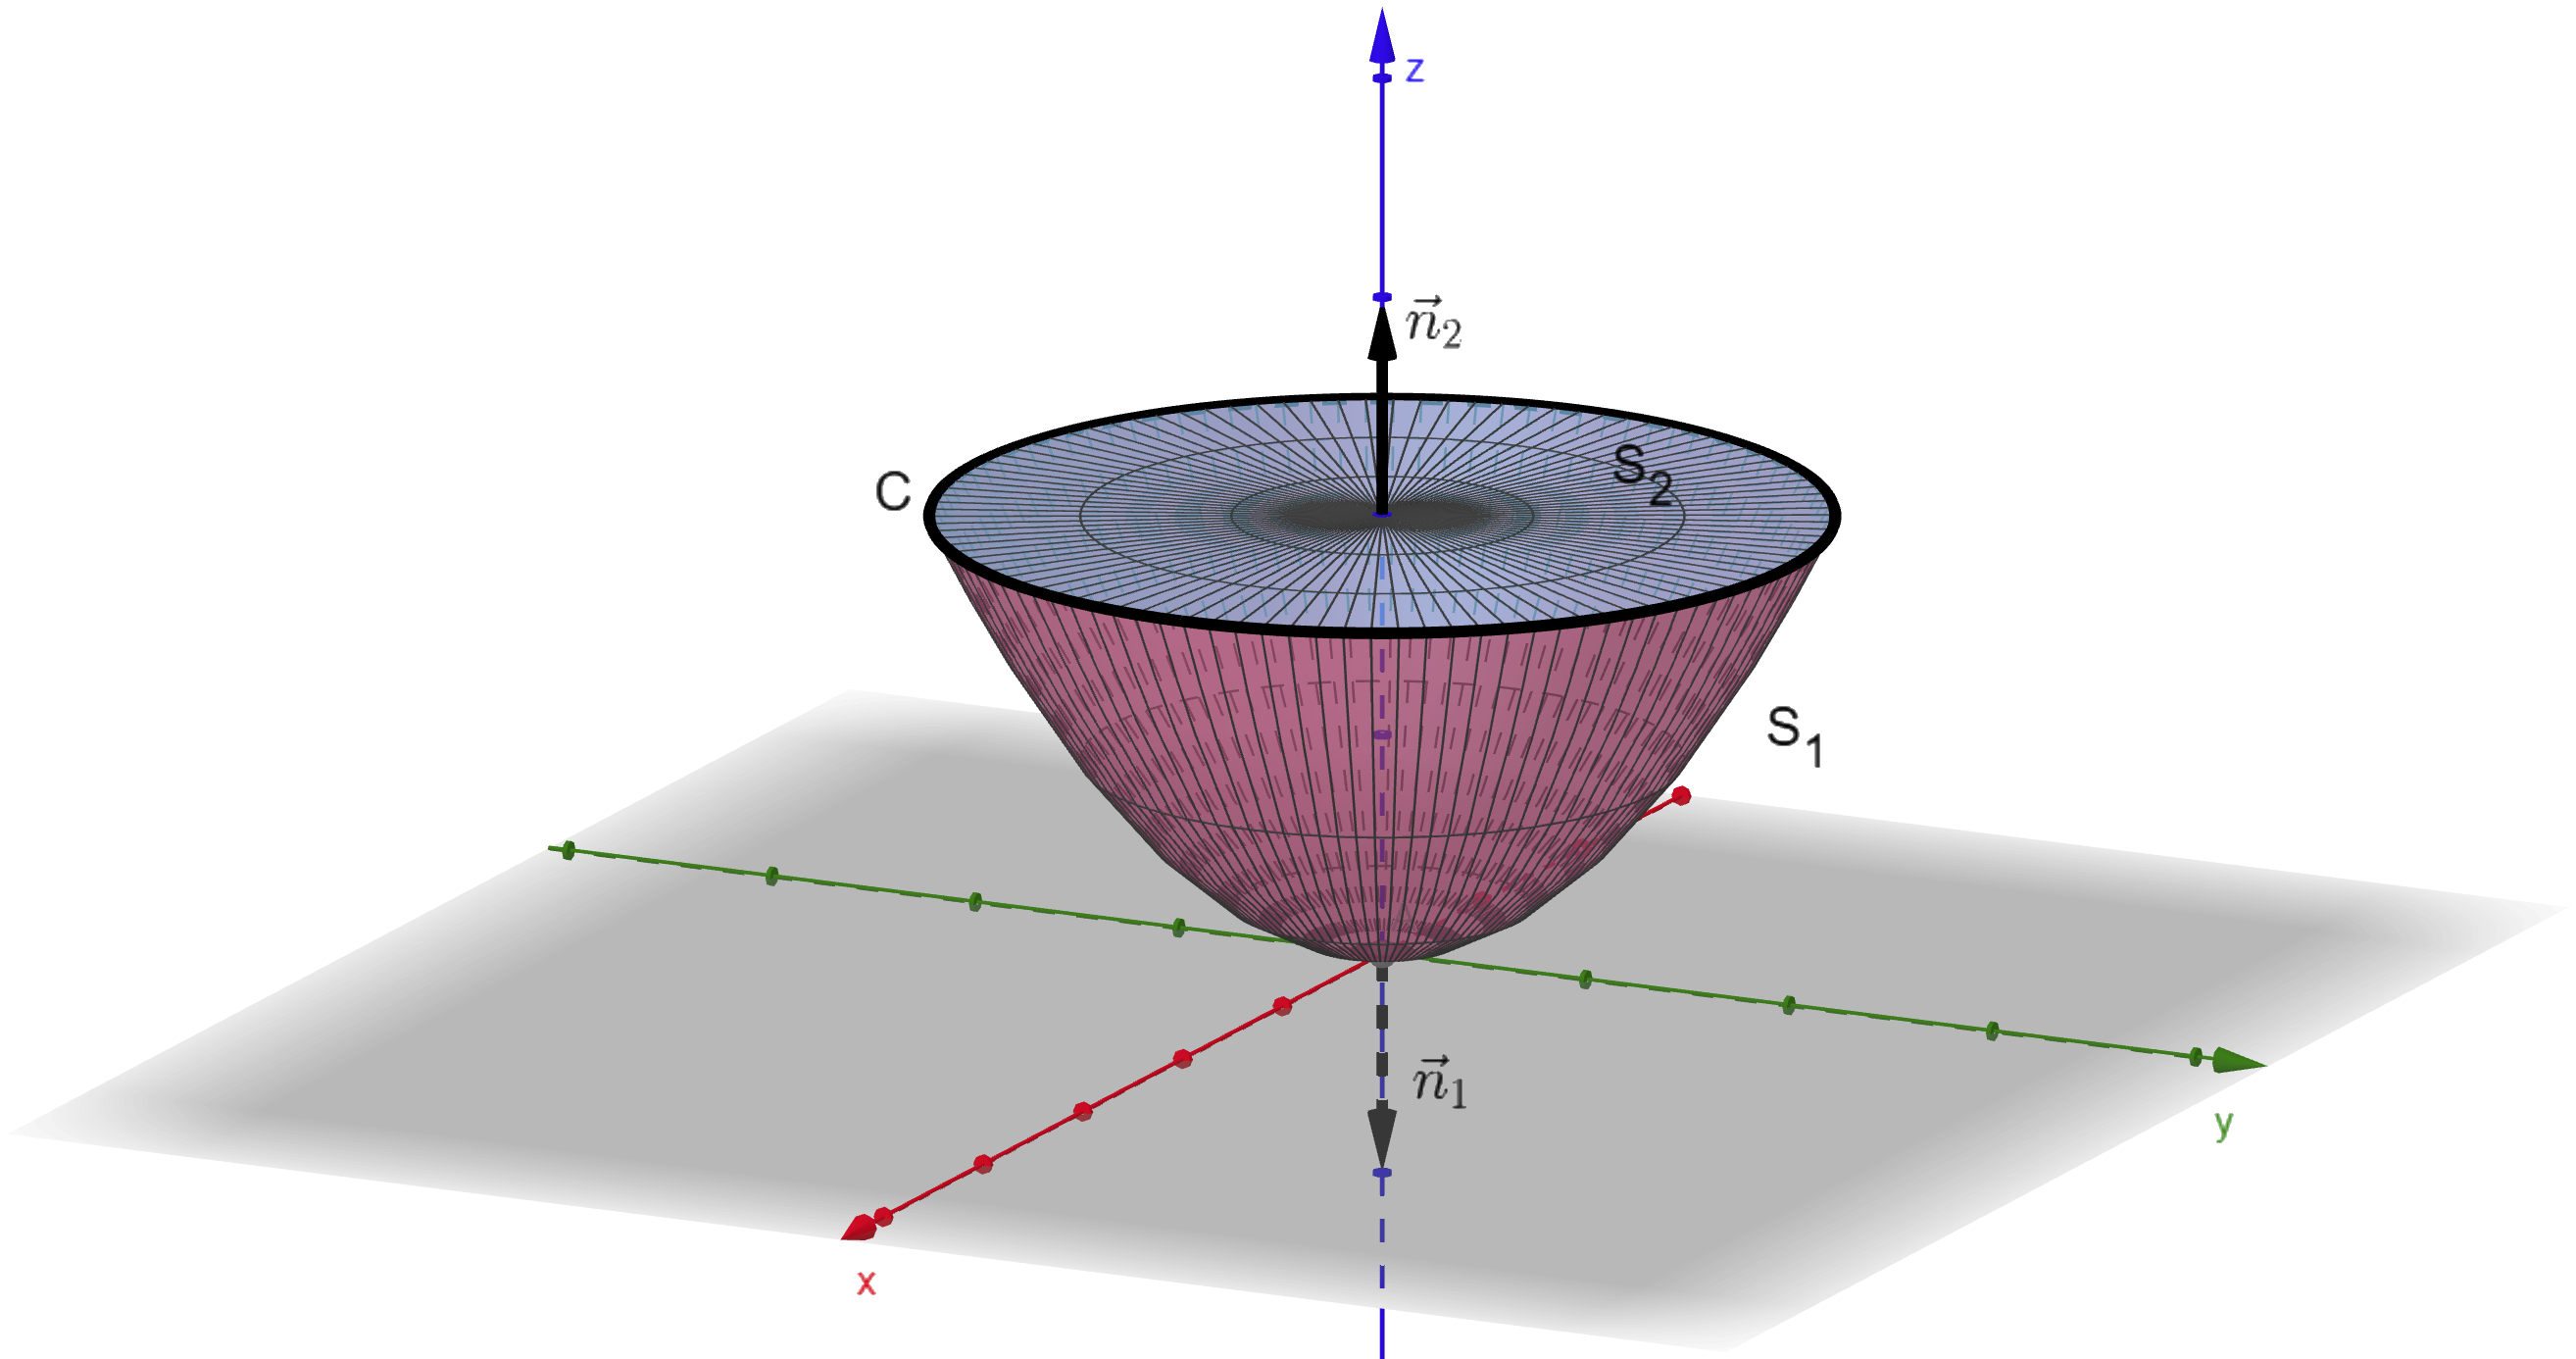
\includegraphics[width=0.65\linewidth]{images/borde2.png}
    \end{center}
    Por la definición anterior de la integral de superficie orientada, tenemos que
    \[
        \int_{(S, \vec{n})} \vec{F} = \int_{(S_1, \vec{n}_1)} \vec{F} + \int_{(S_2, \vec{n}_2)} \vec{F}
    \]
    Comenzamos definiendo el dominio para las parametrizaciones de $S_1$ y $S_2$:
    \[
        \overline{D} = \{(x,y) \in \mathbb{R}^2 \mid x^2 + y^2 \leq 1\}
    \]
    La parametrización de $S_1$ es:
    \[
        \varphi_1 : \overline{D} \to S_1, \quad \varphi_1(x,y) = (x, y, x^2 + y^2)
    \]
    Calculamos la normal:
    \[
        \vec{N}_{\varphi_1} =
        \begin{vmatrix}
            \vec{e}_1 & \vec{e}_2 & \vec{e}_3 \\
            1         & 0         & 2x        \\
            0         & 1         & 2y
        \end{vmatrix}
        = (-2x, -2y, 1)
    \]
    Evaluando la función $\varphi_1$ en el origen obtenemos que $\varphi_1(0,0) =
        (0,0,1)$ que apunta hacia arriba, es decir, en sentido opuesto al vector normal
    $\vec{n}_1 = (0,0,-1)$, luego $\vec{n}_1 = -\vec{N}_{\varphi_1}$.\\ Calculamos
    la integral del campo vectorial sobre la superficie $(S_1, \vec{n}_1)$:
    \[
        \int_{(S, \vec{n}_1)} \vec{F} = \int_{D} \langle \vec{F}(\varphi_1(x,y)), \vec{N}_{\varphi_1}(x,y) \rangle dx dy = -\int_{D} \langle (x(x^2+y^2), y(x^2+y^2), 0), (-2x, -2y, 1) \rangle dx dy
    \]
    \[
        = 2\int_{\theta = 0}^{\theta=2\pi} \int_{r=0}^{r=1} r^4 \cdot r \, dr \, d\theta = 4\pi \left[ \frac{r^6}{6} \right]_{r=0}^{r=1} = \frac{4\pi}{6} = \frac{2\pi}{3}
    \]
    Para la parametrización de $S_2$ tenemos:
    \[
        \varphi_2 : \overline{D} \to S_2, \quad \varphi_2(x,y) = (x, y, 1)
    \]
    Calculamos la normal:
    \[
        \vec{N}_{\varphi_2} =
        \begin{vmatrix}
            \vec{e}_1 & \vec{e}_2 & \vec{e}_3 \\
            1         & 0         & 0         \\
            0         & 1         & 0
        \end{vmatrix}
        = (0, 0, 1)
    \]
    Al igual que antes, evaluando la función $\varphi_2$ en el origen obtenemos que
    $\varphi_2(0,0) = (0,0,1)$ que apunta hacia arriba, es decir, en el mismo
    sentido que el vector normal $\vec{n}_2 = (0,0,1)$, luego $\vec{n}_2 =
        \vec{N}_{\varphi_2}$.\\ Procedemos a calcular la integral del campo vectorial
    sobre la superficie $(S_2, \vec{n}_2)$:
    \[
        \int_{(S, \vec{n}_2)} \vec{F} = \int_{D} \langle \vec{F}(\varphi_2(x,y)), \vec{N}_{\varphi_2}(x,y) \rangle dx dy = \int_{D} \langle (x,y,0), (0,0,1) \rangle dx dy = \int_{D} 0 \, dx dy = 0
    \]
    Por lo tanto, la integral de superficie de $\vec{F}$ sobre $S$ es:
    \[
        \int_{(S, \vec{n})} \vec{F} = \frac{2\pi}{3} + 0 = \frac{2\pi}{3}
    \]
}


\ejemplo{
    Sea la superficie $S = S_1 \cup S_2$, donde:
    $$
        S_1 = \{(x,y,z) \in \mathbb{R}^3 : x^2 + y^2 = z^2, \ z \in [1,2] \}
        \qquad
        S_2 = \{(x,y,z) \in \mathbb{R}^3 : z = 2, \ x^2 + y^2 \leq 4 \}
    $$
    y el campo vectorial $\vec{F}(x,y,z) = (x, y, -z)$. Queremos calcular $\int_{(S, \vec{n})} \vec{F}$, donde $\vec{n}$ es la normal exterior.
    \begin{center}
        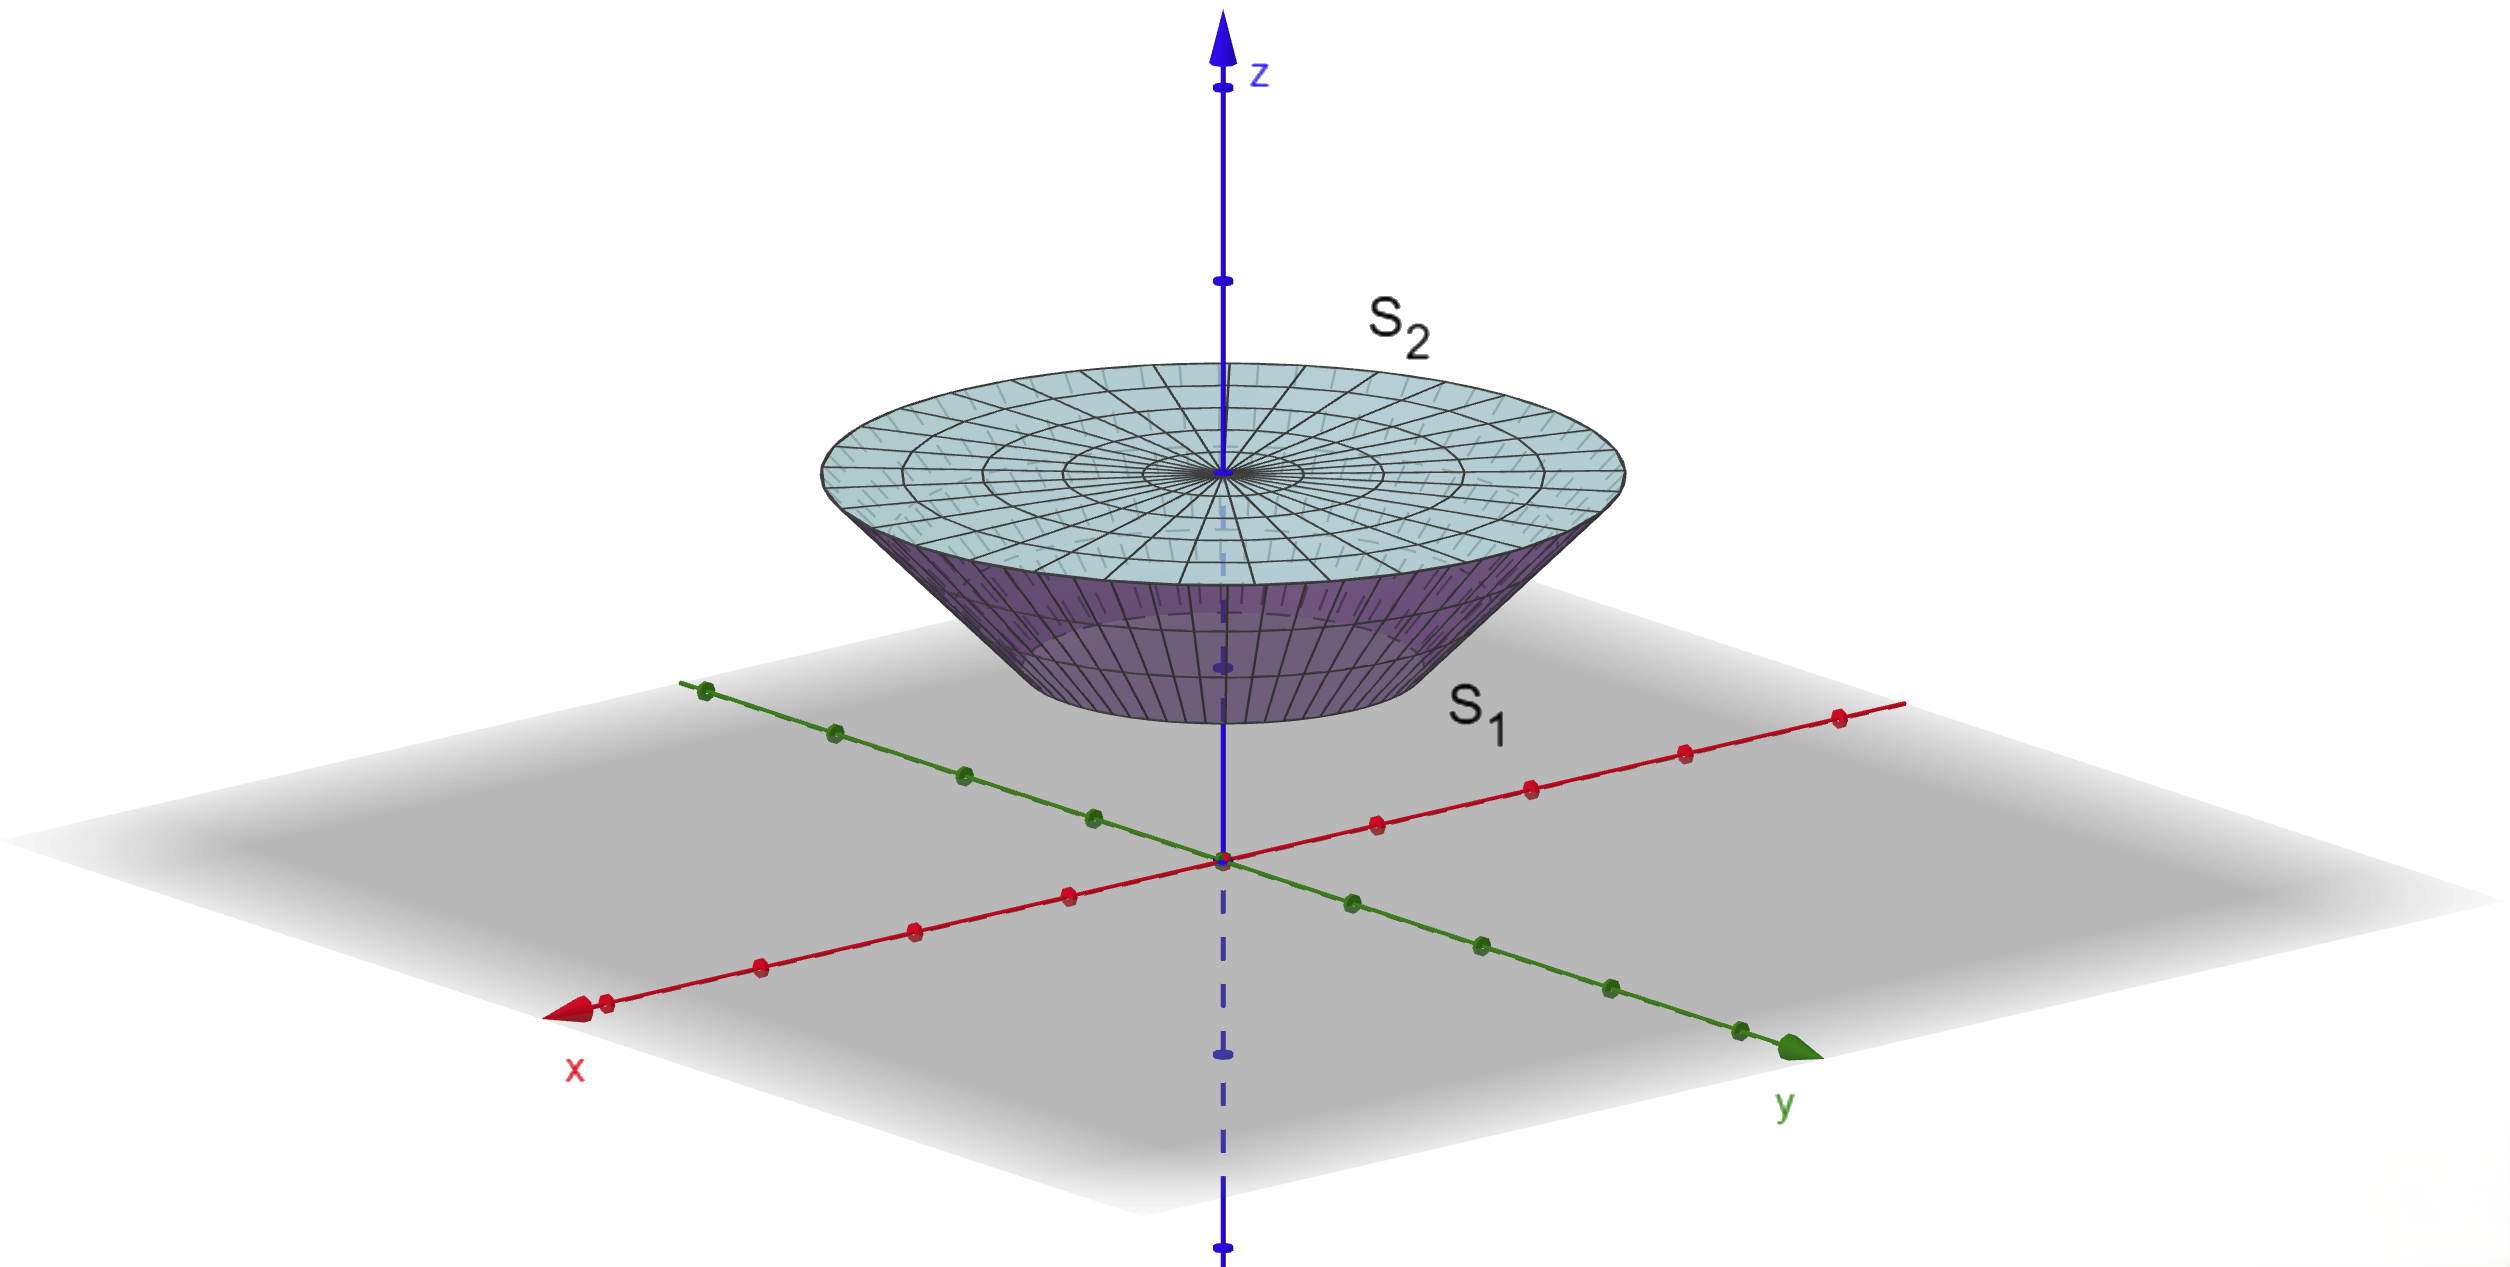
\includegraphics[width=0.65\linewidth]{images/ej3.png}
    \end{center}    
    Observemos que $(S_1, \vec{n}_1)$ y $(S_2, \vec{n}_2)$ tienen orientaciones compatibles, con lo cual $(S, \vec{n})$ está bien orientada.\\
    $$ \int_{(S, \vec{n})} \vec{F} = \int_{(S_1, \vec{n}_1)} \vec{F} + \int_{(S_2, \vec{n}_2)} \vec{F} $$
    Comenzamos parametrizando la superficie $S_1$ con la función $\varphi_1 : D \to S_1$ dada por:
    $$ \varphi_1(r,\theta) = \begin{cases}
        x = r \cos(\theta) \\
        y = r \sin(\theta) \\
        z = r
    \end{cases} \qquad \text{donde } D = \{(r,\theta) \in \mathbb{R}^2 : 1 \leq r \leq 2, \ 0 \leq \theta < 2\pi\} $$
    Calculamos la normal:
    $$ \vec{N}_{\varphi_1} =
        \begin{vmatrix}
            \vec{e}_1 & \vec{e}_2 & \vec{e}_3 \\
            -z \sin(\theta) & z \cos(\theta) & 0 \\
            \cos(\theta) & \sin(\theta) & 1
        \end{vmatrix} = (z \cos(\theta), z \sin(\theta), -z)$$
    Teniendo en cuenta la geometría de la figura y que el vector $\vec{N}_{\varphi_1}$ apunta hacia abajo, entonces es exterior a $S$, luego los vectores $\vec{n}_1$ y $\vec{N}_{\varphi_1}$ son compatibles.\\
    Entonces la integral de $\vec{F}$ sobre $S_1$ es:
    $$ \int_{(S_1, \vec{n}_1)} \vec{F} = \int_{D} \langle \vec{N}_{\varphi_1}, \vec{F} \circ \varphi_1 \rangle = \int_{z=0}^{z=2} \int_{\theta = 0}^{\theta = 2\pi} \langle (z \cos(\theta), z \sin(\theta), -z), (z \cos(\theta), z \sin(\theta), -z) \rangle d\theta dz$$
    $$ = \int_{z=1}^{z=2} \int_{\theta = 0}^{\theta = 2\pi} z^2 + z^2 d\theta dz = 2 \pi \int_{z=1}^{z=2} 2z^2 dz = 4 \pi \left[ \frac{z^3}{3} \right]_{z=1}^{z=2} = 4 \pi \left( \frac{8}{3} - \frac{1}{3} \right) = 4 \pi \cdot \frac{7}{3} = \frac{28\pi}{3}$$
    Ahora consideramos la parametrización $\varphi_2 : E \to S_2$ de $S_2$ dada por:
    $$ \varphi_2 (x,y) = \begin{cases}
        x = x\\
        y = y\\
        z = 2
        \end{cases} \qquad \text{donde } E = \{(x,y) \in \mathbb{R}^2 : x^2 + y^2 \leq 4\}
    $$
    Calculamos la normal:
    $$ \vec{N}_{\varphi_2} =
        \begin{vmatrix}
            \vec{e}_1 & \vec{e}_2 & \vec{e}_3 \\
            1 & 0 & 0 \\
            0 & 1 & 0
        \end{vmatrix} = (0, 0, 1)$$
    La normal $\vec{N}_{\varphi_2}$ apunta hacia arriba, es decir, hacia el exterior de $S$, luego $\vec{n}_2$ y $\vec{N}_{\varphi_2}$ son compatibles.\\
    Entonces la integral de $\vec{F}$ sobre $S_2$ es:
    $$ \int_{(S_2, \vec{n}_2)} \vec{F} = \int_{E} \langle \vec{N}_{\varphi_2}, \vec{F} \circ \varphi_2 \rangle = \int_{x=0}^{x=2} \int_{y=0}^{y=2\pi} \langle (0, 0, 1), (x, y, -z) \rangle dy dx$$
    $$ = \int_{x=0}^{x=2} \int_{y=0}^{y=2\pi} -z dy dx = -2\pi \int_{x=0}^{x=2} 2 dx = -4\pi \left[ x \right]_{x=0}^{x=2} = -4\pi (2-0) = -8\pi$$
    Finalmente, la integral de $\vec{F}$ sobre $S$ es:
    $$ \int_{(S, \vec{n})} \vec{F} = \int_{(S_1, \vec{n}_1)} \vec{F} + \int_{(S_2, \vec{n}_2)} \vec{F} = \frac{28\pi}{3} - 8\pi = \frac{28\pi}{3} - \frac{24\pi}{3} = \frac{4\pi}{3} $$
    
}


\begin{proposición}
    Sea $D = Int(C)$ la parte interior de una curva de Jordan $C$ en $\mathbb{R}^2$ y sea $f : U \to \mathbb{R}$ una función de clase $C^1$ definida en un abierto $U \supset \overline{D}$. Consideramos la superficie $S = G_f$.\\
    Para cada (x,y) en $D$, sea $\theta(x,y)$ el ángulo que forma el vector normal $\vec{n}(x,y)$ a la superficie $S$ en el punto $(x,y,f(x,y))$ con el vector vertical $\vec{e}_3 = (0,0,1)$. Entonces se tiene que:
    $$ a(S) = \int_{D} \frac{dxdy}{\cos(\theta(x,y))}$$
\end{proposición}

\begin{proof}
    Consideramos la parametrización $\varphi : D \to S$ de $S$ dada por:
    $$ \varphi(x,y) = \begin{cases}
        x = x \\
        y = y \\
        z = f(x,y)  
    \end{cases} \qquad \text{donde } (x,y) \in D$$
    Entonces, la normal a la superficie $S$ es:
    $$ \vec{N}_\varphi = \begin{vmatrix}
        \vec{e}_1 & \vec{e}_2 & \vec{e}_3 \\
        1         & 0         & \frac{\partial f}{\partial x} \\
        0         & 1         & \frac{\partial f}{\partial y} \\
    \end{vmatrix} = \left( -\frac{\partial f}{\partial x}, -\frac{\partial f}{\partial y}, 1 \right)$$
    Haciendo el producto escalar con el vector vertical $\vec{e}_3$:
    $$ \langle \vec{N}_\varphi, \vec{e}_3 \rangle = \left( -\frac{\partial f}{\partial x}, -\frac{\partial f}{\partial y}, 1 \right) \cdot (0,0,1) = 1$$
    $$ \langle \vec{N}_\varphi, \vec{e}_3 \rangle = ||\vec{N}_\varphi|| \cdot ||\vec{e}_3|| \cdot \cos(\theta(x,y)) = ||\vec{N}_\varphi|| \cdot 1 \cdot \cos(\theta(x,y)) \implies \lVert \vec{N}_\varphi \rVert = \frac{1}{\cos(\theta(x,y))}$$
    $$a(S) = \int_{D} \lVert \vec{N}_\varphi \rVert dxdy = \int_{D} \frac{1}{\cos(\theta(x,y))} dxdy$$
\end{proof}

\begin{observación}
    Si $S$ está contenida en un plado cuyo vector normal es $\vec{n}$, entonces tenemos que $\theta(x,y)$ es el ángulo entre $\vec{n}$ y el vector vertical $\vec{e}_3$ para cada $(x,y) \in D$.\\
    En este caso, la integral de superficie se puede expresar como:
    $$ a(S) = \int_{D} \frac{dxdy}{\cos(\theta(x,y))} = \frac{1}{\cos(\theta(x,y))} area(D)$$
\end{observación}

\ejemplo{
    Sean los vectores $\vec{u}, \vec{v} \in \mathbb{R}^3$ no nulos, y sea $S$ el paralepípedo definido por los vectores $\vec{u}$ y $\vec{v}$. Entonces el área de la superficie $S$ es:
    $$ a(S) = \lVert \vec{u} \times \vec{v} \rVert = \lVert \vec{u} \rVert \cdot \lVert \vec{v} \rVert \cdot \sin(\theta) $$
    donde $\theta$ es el ángulo entre los vectores $\vec{u}$ y $\vec{v}$.\\
    En efecto, si consideramos la parametrización $\varphi : D \to \mathbb{R}^3$ de $S$ dada por:
    $$ \varphi (\lambda, \mu) = \lambda \vec{u} + \mu \vec{v} \qquad D = \{(\lambda, \mu) \in \mathbb{R}^2 : 0 \leq \lambda, \mu \leq 1\}$$
    entonces tenemos que
    $$ \varphi(\lambda, \mu) = \begin{cases}
        x = \lambda u_1 + \mu v_1 \\
        y = \lambda u_2 + \mu v_2 \\
        z = \lambda u_3 + \mu v_3
    \end{cases}$$
    Calculamos la normal:
    $$ \vec{N}_\varphi =
        \begin{vmatrix}
            \vec{e}_1 & \vec{e}_2 & \vec{e}_3 \\
            u_1 & u_2 & u_3 \\
            v_1 & v_2 & v_3
        \end{vmatrix} = \vec{u} \times \vec{v}$$
    entonces el área de la superficie $S$ es:
    $$ a(S) = \int_{D} \lVert \vec{N}_\varphi \rVert dxdy = \int_{0}^{1} \int_{0}^{1} \lVert \vec{u} \times \vec{v} \rVert d\lambda d\mu = \lVert \vec{u} \times \vec{v} \rVert \int_{0}^{1} d\lambda \int_{0}^{1} d\mu = \lVert \vec{u} \times \vec{v} \rVert$$
}


\begin{observación}
    En $\mathbb{R}^3$, el volumen del paralepípedo definido por los vectores $\vec{u}, \vec{v}, \vec{w} \in \mathbb{R}^3$ es el producto mixto:
    $$ V = \langle \vec{u} \times \vec{v}, \vec{w} \rangle = \begin{vmatrix}
        u_1 & u_2 & u_3 \\
        v_1 & v_2 & v_3 \\
        w_1 & w_2 & w_3
    \end{vmatrix}$$
\end{observación}

\subsection{Teorema de Stokes}

\begin{definición} [Rotacional]
    Sean $A \subset \mathbb{R}^3$ un conjunto abierto y $\vec{F} : A \to \mathbb{R}^3$ un campo vectorial de clase $C^1$. Se define el rotacional de $\vec{F} = (F_1,F_2,F_3)$ como:
    $$ \nabla \times \vec{F} = \begin{vmatrix}
        \vec{e}_1 & \vec{e}_2 & \vec{e}_3 \\
        \frac{\partial}{\partial x} & \frac{\partial}{\partial y} & \frac{\partial}{\partial z} \\
        F_1 & F_2 & F_3
        \end{vmatrix} = \left( \frac{\partial F_3}{\partial y} - \frac{\partial F_2}{\partial z}, \frac{\partial F_1}{\partial z} - \frac{\partial F_3}{\partial x}, \frac{\partial F_2}{\partial x} - \frac{\partial F_1}{\partial y} \right)
    $$
\end{definición}

\begin{observación}
    En este caso, $rot(\vec{F})$ es un campo vectorial continuo definido en $A$.
\end{observación}

\ejemplo{
    Sea $(P,Q) : U \to \mathbb{R}^2$ un campo vectorial de clase $C^1$ definido en un abierto $U \subset \mathbb{R}^2$. Consideramos $A = U \times \mathbb{R}$ y el campo vectorial $\vec{F} = (P,Q,0)$. Entonces el rotacional de $\vec{F}$ es:
    $$ \nabla \times \vec{F} = \begin{vmatrix}
        \vec{e}_1 & \vec{e}_2 & \vec{e}_3 \\
        \frac{\partial}{\partial x} & \frac{\partial}{\partial y} & \frac{\partial}{\partial z} \\
        P & Q & 0
    \end{vmatrix} = \left( 0, 0, \frac{\partial Q}{\partial x} - \frac{\partial P}{\partial y} \right) \text{"la derivación del toerema de Green"}$$
}

\begin{teorema} [Teorema de Stokes]
    Sea $(S, \vec{n})$ una superficie orientada y regular a trozos, y sea $\vec{F}$ un campo vectorial de clase $C^1$ definido en un abierto $U \supset S$. Entonces se cumple la siguiente igualdad:
    $$ \int_{(S, \vec{n})} rot(\vec{F}) = \int_{\partial S} \vec{F} $$
    donde $\partial S$ tiene la orientación inducida por $\vec{n}$.
\end{teorema}

\ejemplo{
    Sea la superficie $S = \{(x,y,z) \in \mathbb{R}^3 : z = x^2 + y^2 \leq 4\}$ con la norma exterior $\vec{n}$ y el campo vectorial $\vec{F} = (yz, -xz, z)$. Verificamos el teorema de Stokes.\\
    Tenemos que $\partial S = \{(x,y,z) \in \mathbb{R}^3 : z = x^2 + y^2 = 4\}$, que es un círculo de radio 2.\\
    El rotacional de $\vec{F}$ es:
    $$ rot(\vec{F}) = \nabla \times \vec{F} = \begin{vmatrix}
        \vec{e}_1 & \vec{e}_2 & \vec{e}_3 \\
        \frac{\partial}{\partial x} & \frac{\partial}{\partial y} & \frac{\partial}{\partial z} \\
        yz & -xz & z
    \end{vmatrix} = \left( x, y, -2z \right)$$
    Consideramos la parametrización natural $\varphi : D \to S$ de $S$ dada por:
    $$ \varphi(x,y) = \begin{cases}
        x = x \\
        y = y \\
        z = x^2 + y^2
    \end{cases} \qquad \text{donde } D = \{(x,y) \in \mathbb{R}^2 : x^2 + y^2 \leq 4\}$$
    Entonces la normal a la superficie $S$ es:
    $$ \vec{N}_\varphi =
        \begin{vmatrix}
            \vec{e}_1 & \vec{e}_2 & \vec{e}_3 \\
            1         & 0         & 2x        \\
            0         & 1         & 2y
        \end{vmatrix} = (-2x, -2y, 1)$$
    La normal $\vec{N}_\varphi$ apunta hacia arriba en el punto $(0,0,0)$, luego tenemos una normal interior.
    \begin{itemize}
        \item $$\int_{(S, \vec{n})} rot(\vec{F}) = \int_{D} \langle \vec{N}_\varphi, rot(\vec{F}) \circ \varphi(x,y) \rangle dx dy = \int_{D} \langle (-2x, -2y, 1), (x,y,-2(x^2+y^2) \rangle dx dy$$
        $$ = \int_{D} 2x^2 + 2y^2 + 2x^2 + 2y^2 dx dy = \int_{D} 4(x^2+y^2) dx dy = 4 \int_{\theta=0}^{\theta=2\pi} \int_{r=0}^{r=2} r^2 \cdot r \, dr \, d\theta$$ 
        $$= 4 \cdot 2\pi \left[ \frac{r^4}{4} \right]_{r=0}^{r=2} = 4 \cdot 2\pi \cdot 4 = 32\pi$$
        \item $$\int_{\partial S} \vec{F} = \int_{C^-} \vec{F} = -\int_{\gamma} \vec{F} = -\int_{t=0}^{t=2\pi} \langle (8 \sin(t), -8 \cos(t), 4), (-2 \sin(t), 2 \cos(t), 0) \rangle dt$$
        $$= \int_{t=0}^{t=2\pi} 16 dt = 16 \left[ t \right]_{t=0}^{t=2\pi} = 16(2\pi - 0) = 32\pi$$
    \end{itemize}
}

\ejemplo{
    Sea $S = S_1 \cup S_2$, donde:
    $$
        S_1 = \{(x,y,z) \in \mathbb{R}^3 : x^2 + y^2 = 1, \ z \in [0,2] \}
        \qquad
        S_2 = \{(x,y,z) \in \mathbb{R}^3 : z = 2, \ x^2 + y^2 \leq 1 \}
    $$
    con la norma exterior $\vec{n}$ y el campo vectorial $\vec{F}(x,y,z) = (y,x,z)$. 
    El borde de $S$ es:
    $$ \partial S = C_0^+ = \{(x,y,z) \in \mathbb{R}^3 : x^2 + y^2 = 1, \ z = 0 \}$$
    Calculamos el rotacional del campo $\vec{F}$:
    $$ rot(\vec{F}) = \nabla \times \vec{F} = \begin{vmatrix}
        \vec{e}_1 & \vec{e}_2 & \vec{e}_3 \\
        \frac{\partial}{\partial x} & \frac{\partial}{\partial y} & \frac{\partial}{\partial z} \\
        y & x & z
    \end{vmatrix} = \left( 0, 0, 1 - 1 \right) = (0,0,0)$$
    Consideramos la parametrización $\gamma$ de la curva $C_0$ dada por:
    $$ \gamma(t) = \begin{cases}
        x = \cos(t) \\
        y = \sin(t) \\
        z = 0
    \end{cases} \qquad \text{donde } t \in [0,2\pi]$$
    que tiene orientacion positiva. Además, $\gamma'(t) = (-\sin(t), \cos(t), 0)$.
    \begin{itemize}
        \item $$\int_{(S, \vec{n})} rot(\vec{F}) = \int_{(S_1, \vec{n}_1)} \vec{0} = 0$$
        \item $$\int_{\partial S} \vec{F} = \int_{C_0^+} \vec{F} = \int_{t=0}^{t=2\pi} \langle (\sin(t), \cos(t), 0), (-\sin(t), \cos(t), 0) \rangle dt$$
        $$= \int_{t=0}^{t=2\pi} \cos^2(t) - \sin^2(t) dt = \int_{t=0}^{t=2\pi} \cos(2t) dt = \left[ \frac{\sin(2t)}{2} \right]_{t=0}^{t=2\pi} = 0$$
    \end{itemize}
}

\ejemplo{
    Consideramos el campo vectorial $\vec{F} = (yz, -xz, z)$. Veamos el rotacional de $\vec{F}$:
    $$ rot(\vec{F}) = \nabla \times \vec{F} = \begin{vmatrix}
        \vec{e}_1 & \vec{e}_2 & \vec{e}_3 \\
        \frac{\partial}{\partial x} & \frac{\partial}{\partial y} & \frac{\partial}{\partial z} \\
        yz & -xz & z
    \end{vmatrix} = \left( x, y, -2z \right)$$
    Supongamos que tenemos una superficie exótica $S$ cuyo borde sea la curva $C_0^+$ del ejemplo anterior. Entonces tenemos que:
    $$ \int_{(S, \vec{n})} rot(\vec{F}) = \int_{C_0^+} \vec{F} = \int_{C_0^+} \vec{F} = \int_{t=0}^{t=2\pi} \langle (0,0,0), (-\sin(t), \cos(t), 0) \rangle dt = 0$$
}

\begin{observación}
    Si $S$ es una superficie cerrada, es decir, $\partial S = \emptyset$, entonces se tiene que:
    $$ \int_{(S, \vec{n})} rot(\vec{F}) = \int_{\partial S} \vec{F} = 0$$
\end{observación}